%-------------------- --------------------
%------  -------------------
%-------------------- --------------------

%%% HEADER einbinden %%%
%-------------------- --------------------
%---------- header.tex -------------------
%-------------------- --------------------

\documentclass[
	ngerman,
	a5paper,
	twoside,
	fontsize=9pt,
	notitlepage,
	DIV=9,
	%DIV=calc
	%headings=small,
	%twocolumn,
	%openany,
	version=last,  % neueste Version - Für Rückwärtskompatibilität hier die gewünschte Version eintragen.
]{scrartcl} % scrartcl

%\usepackage[l2tabu, orthodox]{nag} % auf schlechten Code prüfen

%-------------------- --------------------
%------- Pakete laden  -------------------
%-------------------- --------------------
\usepackage{etex}	% damit mit TIKZ kein Fehler "`No room for a new \dimen"' auftaucht.
%%\usepackage 								{fixltx2e} 	% not required with latex version later than 2015
\usepackage [T1] 						{fontenc} 
\usepackage 								{lmodern}
\usepackage [utf8] 					{inputenc}	% (utf8, ansinew, latin1, applemac)
\usepackage [ngerman]				{babel}	
\usepackage 								{ragged2e}	
%\usepackage [babel]					{microtype}

\usepackage{xifthen}
	\newboolean{a5} 	
	%\setboolean{a5}{false}
	\setboolean{a5}{true}

% Layout etc.
\usepackage [singlespacing]	{setspace}
\usepackage [left=1.6cm, right=1cm, top=0.5cm, bottom=00cm, includeheadfoot]	{geometry}
\usepackage									{multicol}
%\usepackage [above, below]	{placeins}
\usepackage[babel]{microtype}

% Formatierungen u.ä.
\usepackage [dvipsnames]		{xcolor}
\usepackage [normalem]			{ulem}
\usepackage									{fancybox}
\usepackage [hyphens]				{url}
\usepackage									{textcomp}

% Mathematik
\usepackage{nicefrac}
\usepackage{amsmath}			
\usepackage{amssymb} 		
\usepackage{mathtools}

% Grafiken
\usepackage{graphicx}	
\usepackage{wrapfig}
\usepackage[hypcap=false]{caption} % hypcap=false, damit die Warnung verschwindet
\usepackage{subcaption}
\usepackage{tikz}
%\usepackage{pgf}

% Tabellen
\usepackage{booktabs}
\usepackage{tabularx}
	%--- Tabularx konfigurieren  -----------
	%Tabellenausrichtung mit Breite-Angabe ermöglichen
	\newcolumntype{L}[1]{>{\RaggedRight \arraybackslash}p{#1}} % linksbündig	%mit tabularx neue Spaltentypen definieren.
	\newcolumntype{M}[1]{>{\RaggedRight \arraybackslash}m{#1}} % linksbündig
	
	\newcolumntype{C}[1]{>{\Centering \arraybackslash}p{#1}} % zentriert
	\newcolumntype{D}[1]{>{\Centering \arraybackslash}m{#1}} % zentriert
		
	\newcolumntype{R}[1]{>{\RaggedLeft \arraybackslash}p{#1}} % rechtsbündig
	
	\newcolumntype{B}[1]{>{\arraybackslash}p{#1}}	%Blocksatz
	%% %% %% %% %% %% %% 
%--------------------------
\usepackage{colortbl}
\usepackage{longtable}
\usepackage{hhline}

% ANDERES
\usepackage{blindtext} 
%\usepackage{pgfplots}
%\usepackage{filecontents}
%\usepackage{enumitem}
\usepackage{xspace}
\usepackage{calc}
\usepackage{scrlayer-scrpage}
%%\usepackage{titlesec}
\usepackage{boxedminipage}


%-------------------- --------------------
%-------------- Listings -----------------
%-------------------- --------------------
\usepackage{listings}
\lstset{literate=%	% Für utf8 notwendig.
	{Ö}{{\"O}}1
	{Ä}{{\"A}}1
	{Ü}{{\"U}}1
	{ß}{{\ss}}1
	{ü}{{\"u}}1
	{ä}{{\"a}}1
	{ö}{{\"o}}1
	{–}{{-}}1			% falls versehentlich – hereinkopiert wird.
	%{~}{{\textasciitilde }}1
}
%\lstset{texcl=true}

%%%
% Farbig markieren:
% - Befehle			(Standard) - erledigt	(blau)
% - Pakete			(teal - grün)
% - Umgebungen	(purple)
% - Längenmaße	
%%%
\lstset{
		keywordstyle=\color{NavyBlue},		% Befehle	% NavyBlue
		emphstyle=[1]{\bfseries\color{purple}},		% Pakete
		emphstyle=[2]{\bfseries\color{teal}},	% Umgebungen
		emphstyle=[3]{\bfseries\color{teal}},	% Längenmaße
}
\lstset{
	numbers			=none,                        % (left, right, none)
	numberstyle	=\tiny,                      	% Line-numbers fonts
	stepnumber	=1,                           % Step between two line-numbers
	numbersep		=5pt,%5pt,       							% How far are line-numbers 
	frame				=none,                        % A frame around the code
	tabsize			=2,                           % Default tab size
	captionpos	=b,                           % Caption-position = bottom
	breaklines	=true,                        % Automatic line breaking?
	breakatwhitespace=false,                	% Automatic breaks only at whitespace?
	showspaces	=false,                       % Dont make spaces visible
	showstringspaces = false									% Leerzeichen in Strings anzeigen
	showtabs		=false,                       % Dont make tabls visible
	columns			=flexible, %flexible,						% Column format  (flexible, fixed or fullflexible)
	%keepspaces=true, 
}

%-----------------------------------------
%% Styles: basicstyle, identifierstyle, commentsyle, stringstyle, keywordstyle
\lstset{
	language		=[LaTeX]{TeX},
	%backgroundcolor=\color{lightgray},
	basicstyle			={\ttfamily\small},
	commentstyle		={\ttfamily\color{darkgray}},
	identifierstyle	={\ttfamily},
	stringstyle			={\ttfamily},
}

%-----------------------------------------
\lstset{
	%keywordstyle=\ttfamily,
	%keywordstyle=\color{blue},		% Keywords font ('*' = uppercase)
	otherkeywords={}, 
	deletekeywords={}
}
%-------- morekeywords -------------------------

%----- morekeywords: Basic LaTeX --------------
\lstset{morekeywords={
part, chapter, subsection, subsubsection, addsec,
ftrq, flq, href,
tableofcontents, thechapter, thesection, thetable, thefigure, chaptername,
newblock, 
chaptermarkformat, sectionmarkformat, subsectionmarkformat, thesubsection, chapappifchapterprefix,
autodot,
setlength,
glqq, grqq, frqq, flqq, glq, grq, frq, grq,		% Anführungszeichen
eqref, appendix, marginline,
phantomsection,	
textsubscript,
texorpdfstring,
}}

%----- morekeywords: SONSTIGES --------------
\lstset{morekeywords={
meinBefehl, beispiel, addlinespace, arraybackslash, xspace, nicefrac, themyctr, mylen, VARIABLE, NAME, text,
zB, addtokomafont,
whiledo,
KOMAoptions,
url,
showkeyslabelformat,
linnumbers,
sectfont,
extrarowheight
}}

%----- morekeywords: Mathe (Package amsmath etc.) ------
\lstset{morekeywords={
mathcal, mathbb, mathring, tag, notag
}}

%----- morekeywords: Package Blindtext --------------
\lstset{morekeywords={
blindtext, Blindtext,
}}

%----- morekeywords: Package booktabs --------------
\lstset{morekeywords={
toprule, midrule, bottomrule, cmidrule
}}

%----- morekeywords: Package calc --------------
\lstset{morekeywords={
real, ratio, maxof, minof
}}

%----- morekeywords: Package Caption --------------
\lstset{morekeywords={
subref, subcaptionref, captionof
}}

%----- morekeywords: Package colortbl --------------
\lstset{morekeywords={
arrayrulecolor, columncolor, rowcolor, cellcolor
}}

%----- morekeywords: Package fancybox --------------
\lstset{morekeywords={
shadowbox, doublebox, ovalbox, Ovalbox
}}

%----- morekeywords: Package graphicx --------------
\lstset{morekeywords={
includegraphics
}}

%----- morekeywords: Package hhline --------------
\lstset{morekeywords={
\hhline
}}

%----- morekeywords: Package listings --------------
\lstset{morekeywords={
lstset, lstinline, lstinputlisting
}}

%----- morekeywords: Package longtable --------------
\lstset{morekeywords={
endfirsthead, endhead, endfoot, endlastfoot, 
}}

%----- morekeywords: Package multicols --------------
\lstset{morekeywords={
columnbreak
}}

%----- morekeywords: Package placeins --------------
\lstset{morekeywords={
FloatBarrier
}}

%----- morekeywords: Package ragged2e --------------
\lstset{morekeywords={
RaggedRight, Centering, RaggedLeft
}}

%----- morekeywords: Package scrpage --------------
\lstset{morekeywords={
clearscrheadfoot, clearscrheadings, clearscrplain,
ihead, chead, ohead, ifoot, cfoot, ofoot,
lehead, cehead, rehead, lohead, cohead, rohead, lefoot, cefoot, refoot, lofoot, cofoot, rofoot,
pagemark, automark, headmark, manualmark,
headfont, footfont, pnumfont,
setheadsepline, setfootsepline, setheadtopline, setfootbotline
}}

%----- morekeywords: Package setspace --------------
\lstset{morekeywords={
doublespacing, onehalfspacing, singlespacing, setstretch
}}

%----- morekeywords: Package tabularx --------------
\lstset{morekeywords={
newcolumntype
}}

%----- morekeywords: Package textcomp --------------
\lstset{morekeywords={
texttwelveudash, textthreequartersemdash,
textdblhyphen, textdblhyphenchar, textasteriskcentered, textborn, textpm, texttimes, textdiv, textfractionsolidus, textonequarter, textonehalf, textthreequarters, textdiscount, textperthousand, textpertenthousand, textsurd,
textonesuperior, texttwosuperior, textthreesuperior, textleftarrow, textrightarrow, textuparrow, textdownarrow, textlangle, textrangle, textlbrackdbl, textrbrackdbl, textlquill, textrquill, textbardbl,
textservicemark, textcopyleft, textcircledP, textpilcrow, textcurrency, textreferencemark, textmusicalnote, textleaf,
textmarried, textdivorced, textdied, textordmasculine, textordfeminine, textbrokenbar, textminus, textasciimacron, textlnot, textinterrobang, textinterrobangdown, texttildelow, textasciibreve, textasciicaron, textacutedbl, textgravedbl, textquotesingle, textquotestraightbase, textquotestraightdblbase, textasciigrave, textasciiacute, textasciidieresis, textasciimacron, textlnot, textinterrobang, textinterrobangdown,  texttildelow,  textasciibreve,  textasciicaron,  textacutedbl,  textgravedbl,  textquotesingle,  textquotestraightbase, textquotestraightdblbase,  textasciigrave, textasciiacute, textasciidieresis,
textblank, textmho, textohm, textmu, textbaht, textcelsius, textcolonmonetary textcentoldstyle, textcent, textdong, textestimated, texteuro, textflorin, textguarani, pounds, textlira, textnaira, textnumero, textpeso, textrecipe, textdollaroldstyle, textyen, textwon,
textopenbullet, textdegree, textbigcircle, textcolonmonetary, textcentoldstyle,
}}

%----- morekeywords: Package tikz --------------
\lstset{morekeywords={
usetikzlibrary, tikz, draw, tikzoptions, node, shade, 
}}

%----- morekeywords: Package ulem --------------
\lstset{morekeywords={
uline, uuline, uwave, sout, xout, dashuline, dotuline,
}}

%----- morekeywords: Package xcolor --------------
\lstset{morekeywords={
textcolor, colorbox, fcolorbox, color, pagecolor, definecolor
}}

%----- morekeywords: Package xifthen --------------
\lstset{morekeywords={
newboolean, setboolean, ifthenelse, isodd, lengthtest, isundefined, equal, AND, OR, NOT, newtest, boolean
}}

%-----------------------------------------


%----- morekeywords: Package VORLAGE --------------
\lstset{morekeywords={
%
}}

%-----------------------------------------
\lstset{
	%% Escape to LaTeX:
	mathescape = false, 	% $a=x$ Mathemodus ermoeglichen
	escapechar = {²},		% Buchstabe zum Verlassen und Zurückkehren (LaTeX-Modus)
	% escapeinside={²}{³},	% Alternative zu escapechar
	%escapebegin= {},		% wird zu Beginn des Escape-Modus eingefügt
	%escapeend= {}				% wird zum Ende des Escape-Modus eingefügt
}

%-----------------------------------------
%----- Weitere Betonungen: Pakete -----
\lstset{emph=[1]{
	usepackage
	%amsmath, amssymb, amsthm, array, babel, blindtext, booktabs, calc, caption, colortbl,  enumitem,  fancybox,  fixltx2e,  mathtools,   microtype,  multicol,   natbib,  nicefrac,  pdflscape,  pdfpages,  pgfplots,  picins,  placeins,  ragged2e, scrpage2  , setspace,  subcaption,  siunitx,  stfloats,  tabularx,  textcomb,  tikz,  url,  ulem,  units,  wrapfig,  xcolor,  xspace, 
}}
%----- Weitere Betonungen: Umbegungen -----
\lstset{
emph=[2]{
	begin, end,
	%array, document, FlushLeft, FlushRight, Center, raggedright, raggedleft, centering, samepage, minipage, figure, wrapfigure, itemize, enumerate, description, tabbing, tabular, lstlisting, math, equation, multline, gather, align, flalign, multicols, landscape, thebibliography,longtable,
},
%emphstyle=[1]{\bfseries\color{purple}}
}

%----- Weitere Betonungen: Längenmaße -----
\lstset{emph=[3]{
	mm, cm, in, pt, em, ex,
}}

%-----------------------------------------
%------------- Listings Ende --------------

\usepackage[pdftex,
	hidelinks,
	pdfauthor=	{cax}, % Autorname
	pdfkeywords={},	% Schluesselwoerter
	pdfdisplaydoctitle=true, 
	pdftitle=		{},	% Titel
	pdfsubject=	{}, % Thema
	%colorlinks=false,
	%linkcolor=MidnightBlue,
	%urlcolor=black,
	%citecolor=black,
	%%%
	bookmarksopen=false,
	%pdffitwindow=true,
	pdfpagelayout={SinglePage},	% (SinglePage, OneColumn, TwoColumnLeft, TwoColumnRight, TwoPageLeft, TwoPageRight)
	pdfpagemode={UseNone},	% (UseNone, UseThumbs, UseOutlines, FullScreen, UseOC, UseAttachments)
	%pagebackref 	=true, 	%zurück-Button im Acrobat-Reader
]{hyperref}  % hyperref sollte als letztes Paket eingebunden werden.%Infos unter {http://de.wikibooks.org/wiki/LaTeX-W%C3%B6rterbuch:_hyperref}


%-------------------- --------------------
%-------------- Einstellungen ------------
%-------------------- --------------------
%% ----- scrheadings (ehemals scrpage2 -----
	\pagestyle{scrheadings}

	\newcommand{\standardKopfzeile}{
		\clearpairofpagestyles
		%\setheadsepline{.4pt}
		\ohead[\pagemark]{\pagemark}
		\rehead[\leftmark]{\leftmark}	% linke Seite innen
		\lohead[\rightmark]{\rightmark} % rechte Seite innen
		\automark[subsection]{section}
	}
	\newcommand{\seitenzahlKopfzeile}{
		\clearpairofpagestyles
		\ohead[\pagemark]{\pagemark}
	}
	\newcommand{\leereKopfzeile}{
		\clearpairofpagestyles
	}
	\newcommand{\AnhangKopfzeile}{
		\clearpairofpagestyles
		\ohead[\pagemark]{\pagemark}
	}
	%\standardKopfzeile
	%\seitenzahlKopfzeile
	\leereKopfzeile
%--------------------------

% ----- Kapitelüberschriften formatieren ------
% --> erst nach dem Inhaltsverzeichnis




%\usepackage{titlesec}
%\titleformat{\section}
%{\color{red}\normalfont\Large\bfseries}
%{\color{Blue}\thesection}{1em}{}
%%(siehe auch http://texblog.org/tag/titlesec/)




%\setlength{\headheight}{0pt}%Überschriften direkt unter Kopfzeile
\pagenumbering{Roman} % Römische Seitennummerierung für Vorspann
	
%%% %%% Trennungs-Liste %%% %%%
	\hyphenation{Pa-ket-be-schrei-bung-en Ka-pi-tel}
%%% %%% %%% %%%

\renewcommand*{\sectfont}{\sffamily\bfseries\boldmath} % Mathe in Überschriften

%\raggedbottom % damit der Inhalt einer nicht füllbaren Seite nicht vertikal verteilt wird. (\raggedbottom, \flushbottom)
\raggedcolumns % (\raggedcolumns, \flushcolumns) damit der Inhalt einer nicht füllbaren Spalte (mittels multicol-Package) nicht vertikal verteilt wird.

\setlength{\extrarowheight}{2pt} % Zeilenabstand in Tabllen

%EOF
% befehle.tex
% Eigene Befehle

\newcommand{\Abb}	{Abb.\,}
\newcommand{\etal}	{et\,al.\xspace}
\newcommand{\zB}	{z.\,B.\xspace}
\newcommand{\vgl}	{vgl.\,}
\newcommand{\pfeil}	{$\rightarrow$\xspace}
\newcommand{\Pfeil}	{$\Rightarrow$\xspace}
\newcommand{\Gl}	{Gl.\,}					% Gleichung
\newcommand{\tabbingrule}	{\rule{\linewidth}{0.5\arrayrulewidth}}
%\newcommand{\}	{}
%\newcommand{\}	{}
%\newcommand{\}	{}
%\newcommand{\}	{}
%\newcommand{\}	{}



%----- Einheiten -----
\newcommand{\cl}{\,cl\xspace}
\newcommand{\g}{\,g\xspace}
\newcommand{\mg}{\,mg\xspace}
\newcommand{\ml}{\,ml\xspace}
\newcommand{\Lit}{\,L\xspace}
\newcommand{\kJ}{\,kJ\xspace}
\newcommand{\kcal}{\textcolor{red}{\,kcal}}

\newcommand{\EL}{\,EL\xspace}
\newcommand{\TL}{\,TL\xspace}

%----- Blindtext -----
\newcommand{\Bla}{
	Dies hier ist ein Blindtext zum Testen von Textausgaben. Wer diesen Text liest, ist selbst schuld.
	Der Text gibt lediglich den Grauwert der Schrift an.
	Ist das wirklich so?
	Ist es gleichgültig, ob ich schreibe: „Dies ist ein Blindtext“ oder „Huardest gefburn“? Kjift mitnichten!
	Ein Blindtext bietet mir wichtige Informationen.
	}
\newcommand{\bla}{
	Dies hier ist ein Blindtext zum Testen von Textausgaben.
	}


% ---- red ----
\newcommand
	{\red}
	{\color{red}}
\newcommand
	{\txtred}[1]
	{\textcolor{red}{#1}}
\newcommand
	{\bgred}[1]
	{\colorbox{Salmon}{#1}}

% ---- orange ----
\newcommand
	{\orange}
	{\color{orange}}
\newcommand
	{\txtorange}[1]
	{\textcolor{orange}{#1}}
\newcommand
	{\bgorange}[1]
	{\colorbox{orange}{#1}}

% ---- yellow ----
\newcommand
	{\yellow}
	{\color{yellow}}
\newcommand
	{\txtyellow}[1]
	{\textcolor{yellow}{#1}}
\newcommand
	{\bgyellow}[1]
	{\colorbox{yellow}{#1}}

	
% ----green  ----
\newcommand
	{\green}
	{\color{Green}}
\newcommand
	{\txtgreen}[1]
	{\textcolor{Green}{#1}}
\newcommand
	{\bggreen}[1]
	{\colorbox{lime}{#1}}
	
% ---- blue ----
	\newcommand
	{\blue}
	{\color{Blue}}
\newcommand
	{\txtblue}[1]
	{\textcolor{Blue}{#1}}
\newcommand
	{\bgblue}[1]
	{\colorbox{Cerulan}{#1}}
	
% ---- gray ----
\newcommand
	{\gray}
	{\color{gray}}
\newcommand
	{\txtgray}[1]
	{\textcolor{gray}{#1}}
\newcommand
	{\bggray}[1]
	{\colorbox{lightgray}{#1}}
	
% ----  ----

%----- d/dt  und  d{}/dt -----
\newcommand{\ddt}[1][]	% z.B. \ddt[\phi] oder \ddt
	{\frac{ \mathrm{d}#1 }{\mathrm{d}t}}

%----- dt -----
\newcommand{\dt}
	{\mathrm{d}t}
	
%----- d{} -----
\newcommand{\diff}
	[1]
	{\mathrm{d}#1}

%----- dphi -----	
\newcommand{\dphi}
	{\mathrm{d}\phi}
	

%----- Mathe-Abk�rzungen -----
\newcommand{\Ln}{\mathrm{Ln}}
\newcommand{\arcosh}{\mathrm{arcosh}\,}


%----- Mengen-Symbole -----
\newcommand{\N}{\mathbb{N}}	% Nat�rliche Zahlen (0,1,2,3,..)
\newcommand{\Z}{\mathbb{Z}} % Ganze Zahlen (..,-2,-1,0,1,2,..)
\newcommand{\Q}{\mathbb{Q}} % Rationale Zahlen (Quotienten aus Z)
\newcommand{\R}{\mathbb{R}} % Reelle Zahlen (Q + sqrt(2) etc.)
\newcommand{\C}{\mathbb{C}} % Komplexe Zahlen (1+3*i)
%% Info: \N \in \Z \in \Q \in \R \in \C

% Formatierungsbefehle
\newcommand{\Paket}[1]{\textcolor{purple}{#1}}
\newcommand{\Befehl}[1]{\textcolor{NavyBlue}{#1}}	% (blue, NavyBlue)
\newcommand{\Umgebung}[1]{\textcolor{teal}{#1}}
\newcommand{\Laenge}[1]{\textcolor{teal}{#1}}		
\newcommand{\notiz}{\color{Cerulean}}

% Vereinfachungs-Befehle
\newcommand{\mytitleformat}[1]{\texorpdfstring{#1}{}}
	% verhindert Fehler, wenn Formatierungen im Titel verwendet werden: \section{ \titelformat{\color{red}} TEXT }
\newcommand{\scite}[2]{\cite[S.\,#2]{#1}}	% \scite{Jahne12}{123\,f}

\newcommand{\mycolumnbreak}{\columnbreak} % (\columnbreak,\newpage)
\newcommand{\myHspace}{\hspace{1ex}} % Abstand in Listen Mathematische Symbole
\newcommand{\myhrule}
	{	\vspace{-.5\baselineskip} \hrule }
	
\newcommand{\mminipage}[2]{\begin{minipage}{#1}#2\end{minipage}}
\newcommand{\befehlsformat}[1]
	{%
	{\ttfamily\small\color{NavyBlue} \textbackslash{#1}}%
	}
\newcommand{\todo}[1]{{\textcolor{purple}{TODO: \textasteriskcentered} \color{gray}~#1~\textcolor{purple}{\textasteriskcentered}}}
	
%----- Abstände -----
\newcommand{\negAbstand}{\vspace{-0.55\baselineskip}} % negativer Abstand. Zweck: Abstand zwischen Überschrift und lstlisting-Umgebung oder ähnlichem verringern.
\newcommand{\posAbstand}{\vspace{0.55\baselineskip}}
\newcommand{\negspace}{\negAbstand} % Synonym --> Coolere Befehl
\newcommand{\posspace}{\posAbstand} % Synonym --> Coolere Befehl
\newcommand{\notizenplatz}{\vspace{5\baselineskip}}
\newcommand{\notizenplatzx}{\vspace*{5\baselineskip}}

%-----  ------
%%Befehl \mycirc{..} für Kreis um Buchstaben definieren (usepackage{tikz} notwendig)
%\newcommand*{\mycirc}[1]{ 
	%\begin{tikzpicture}[baseline=(C.base)]%
    %\!\!\!% negativer Abstand
		%\node[draw,circle,inner sep=1pt](C) {#1};
		%\!\!\!%negativer Abstand
  %\end{tikzpicture}
%}


% Development stages (wikibooks.org nachempfunden. vgl. [en.wikibooks.org/wiki/Help:Development_stages])
\newlength{\stageHeight}
\setlength{\stageHeight}{1.5ex}
%\settoheight{\stageHeight}{d}
\newcommand{\stage}[1]{
	\ifcase #1 % 0
		\texorpdfstring{%
			\settoheight{\stageHeight}{R}%
			
\includegraphics[height=\stageHeight,%
			trim={0 0.3mm 0 0}]{Bilder/stage0}%
		}{}%
	\or % 1
		\texorpdfstring{%
			\settoheight{\stageHeight}{R}%
			
\includegraphics[height=\stageHeight,%
			trim={0 0.3mm 0 0}]{Bilder/stage1}%
		}{}%
	\or % 2
		\texorpdfstring{%
			\settoheight{\stageHeight}{R}%
			
\includegraphics[height=\stageHeight,
			trim={0 0.3mm 0 0}]{Bilder/stage2}%
		}{}%
	\or % 3
		\texorpdfstring{%
			\settoheight{\stageHeight}{R}%
			
\includegraphics[height=\stageHeight,%
			trim={0 0.3mm 0 0}]{Bilder/stage3}%
		}{}%
	\or % 4
		\texorpdfstring{%
			\settoheight{\stageHeight}{R}%
			
\includegraphics[height=\stageHeight,%
			trim={0 0.3mm 0 0}]{Bilder/stage4}%
		}{}%
	\else		% >4
		\textcolor{red}{ND}
	\fi
}
% Beschreibung:
%%\begin{description}
	%%\item[\stage{0} Neu]  				Kaum Text
	%%\item[\stage{1} Erstentwurf]  Keine klare Struktur
	%%\item[\stage{2} In Arbeit]		Mittl. -- großer Änd.-bed.
	%%\item[\stage{3} Fortgeschritten]	Geringer Änd.-bed.
	%%\item[\stage{4} Fertig] 	Kein Änderungsbedarf
%%\end{description}
%%Symbole entnommen aus [Wikibooks.org "`Development Stages"' (\url{en.wikibooks.org/wiki/Help:Development_stages})]
\newcommand{\sectionstage}[2][-1]{%
	\section[#2]{#2\stage{#1}}% 	\sectionstage{2}{TITEL}
}
\newcommand{\subsectionstage}[2][-1]{% 
	\subsection[#2]{#2\stage{#1}}% 			\subsectionstage{2}{TITEL}
}
\newcommand{\subsubsectionstage}[2][-1]{% 
	\subsubsection[#2]{#2\stage{#1}}% 	\subsubsectionstage{2}{TITEL}
}
%
\newcommand{\sectionstageS}[2][-1]{% X anstatt von * (irgendwie nicht möglich)
	\section*{#2\stage{#1}}% 	\subsubsectionstage{2}{TITEL}
}
\newcommand{\subsectionstageS}[2][-1]{% 
	\subsection*{#2\stage{#1}}% 	\subsubsectionstage{2}{TITEL}
}
\newcommand{\subsubsectionstageS}[2][-1]{% 
	\subsubsection*{#2\stage{#1}}% 	\subsubsectionstage{2}{TITEL}
}


%%%%%%%%%%%%%%%%%%%%%%%%%%%%%%%%%

%%% Dokument %%%
\begin{document}

\pagenumbering{arabic}

%-------------------- --------------------
%---------- 0_Titelseite.tex -------------
%-------------------- --------------------

\begin{titlepage}
\thispagestyle{empty}
\normalsize

~
\vspace{2cm}
\begin{center} 
\bigskip		
\vspace{4ex}
{\Huge \bfseries \LaTeX2e{} Quick Reference}

%%% ABSTAND %%%
\vspace{15ex}

%%% Titel %%%
\begin{doublespace}% singlespace % onehalfspace % doublespace
{
\Large%
\bfseries% fett
Christoph Axthelm\linebreak
}
\vfill

\begin{FlushLeft}
\textbf{Änderungslog:}  \\
%
\begin{tabbing}
September 2014: ~~~~~\= \kill
August 2014: 		\> Version Beta 2.0\\
Januar 2016: \> Version Beta 2.1: Kleine Layout-Überarbeitungen\\
September 2021:			\> Version Beta 2.2: Interne Korrekturen (Paket-Updates) \\
\end{tabbing}
%
\end{FlushLeft}

\vfill
\vfill
\vfill
%\vspace{50ex}

\end{doublespace}%
\textit{\today \ / Version Beta 2.2}
\end{center}

%%% Linksbündig %%%
\RaggedRight


\vfill

\end{titlepage}

%%% EOF %%%

\setlength{\columnseprule}{0.5pt}



%----- Inhaltsverzeichnis -----
\clearpage
\begin{multicols}{2}
\setcounter{tocdepth}{3} % Tiefe des Inhaltsverzeichnisses
\tableofcontents

\vspace{0.5\baselineskip} 
\hrule

\end{multicols}

%----- Vorwort -----
\clearpage
\standardKopfzeile
\begin{multicols*}{2}

\addtocounter{section}{-1}
%\pagebreak
\sectionstage[3]{Vorwort}
Diese QuickReferenz soll dem schnellen Nachschlagen von \LaTeX-Wissen dienen.
Dabei liegt der Schwerpunkt auf einer besonders kompakten, aber dennoch eindeutigen Darstellungsweise. 
Daher eignet sich die QuickReference vor Allem für fortgeschrittene \LaTeX-Nutzer.
\LaTeX-Einsteiger sollten zunächst einen der zahlreichen sehr guten Einführungskurse durcharbeiten\footnote{Empfehlungen für kostenlose \LaTeX-Einführungen: \cite{l2kurz} (50 Seiten), \cite{Niebler} (416 Vorlesungsfolien), \cite{Quaritsch}}.

%Warum habe ich mir die Mühe für diese QuickReference gemacht? -- Zum einen hat mir eine solche Übersicht selbst gefehlt.
%Zum anderen kann ich damit etwas zur Nutzerfreundlichkeit von \LaTeX beitragen.

Die folgenden Prinzipien werden in der QuickReference verfolgt: 
\begin{itemize}
	\item Zuerst wird das Ergebnis des \LaTeX-Codes gezeigt, dann der zugrunde liegende \LaTeX-Code.
	\item \LaTeX-Befehle werden blau dargestellt\footnote{Ausnahme: Befehle mit Sonderzeichen können leider nicht farblich hervorgehoben werden, da dies vom Paket \Paket{listings} nicht unterstützt wird. 
	Ebenso werden die Schrägstriche  \texttt{\textbackslash} vor den Befehlen nicht hervorgehoben.}:  \lstinline|\LaTeX|.
	\item Pakete werden \Paket{rot} dargestellt.
	Sie müssen im \LaTeX-Code mit \newline\lstinline|\usepackage{Paketname}| geladen werden, \emph{bevor} der Befehl \newline\lstinline|\begin{document}| auftaucht.
	\item Rote Schriftfarbe zeigt an, dass hier Informationen in der QuickReferenz fehlen.
\end{itemize}

\columnbreak
\vspace*{1em}

\noindent
Da die QuickReferenz nicht komplett fertig gestellt wurde, wird zu den Kapiteln und Unterkapiteln mithilfe folgender Symbole%
\footnote{Symbole entnommen aus [Wikibooks.org "`Development Stages"' (\url{http://en.wikibooks.org/wiki/Help:Development_stages})], zuletzt abgerufen am 08.12.2017}
 der Fortschritt des jeweiligen Kapitels angegeben:
\begin{description}
	\item[\stage{0} Neu]  				Kaum Text
	\item[\stage{1} Erstentwurf]  Keine klare Struktur
	\item[\stage{2} In Arbeit]		Mittl. -- großer Änd.-bed.
	\item[\stage{3} Fortgeschritten]	Geringer Änd.-bed.
	\item[\stage{4} Fertig] 	Kein Änderungsbedarf
\end{description}

	%% Bei Kompilierungsfehler diese Zeile vorübergehend auskommentieren.
\hrule

%\columnbreak
%%%% TODO %%%
%\begin{multicols}{2}
%\section*{TODO}
%\begin{enumerate}
	%\item 	
%\end{enumerate}



%\addtolength{\leftmargini}{10pt}
%\ \\
%\ \\
%\ \\
%\end{multicols}
%


\hrule

\end{multicols*}

%----- BEGINN -----
\clearpage
%\begin{multicols*}{2}

\newcommand{\partcolor}{\color{NavyBlue}}

%\standardKopfzeile

\begin{multicols*}{2}
% Befehle definieren
\newcommand{\htmlcb}[1]
{	
	%\textcolor[HTML]{#1}{\rule{1.1em}{2.2ex}} \mbox{\footnotesize #1}
	%\newline
	%\colorbox[HTML]{#1}{#1}
	\textbf{\textcolor[HTML]{#1}{#1}}
}
\newcommand{\colorline}[4]{%
\htmlcb{#1} \htmlcb{#2} \htmlcb{#3} \htmlcb{#4} \newline
}

%\columnbreak
% ----- Kapitelüberschriften formatieren ------
%%Farbset1:
%\addtokomafont{section}{\color[HTML]{3939FC}}
%%Farbset2:

%Farbset ausgeben:
%HTML:
% 841010 844A10 848410 4A8410 
% 84104A BB1616 E62828 108410  
% 841084 28E6E6 16BBBB 10844A
% 4A1084 101084 104A84 108484

%\noindent%
%\colorline{841010}{844A10}{848410}{4A8410}
%\colorline{84104A}{BB1616}{E62828}{108410}
%\colorline{841084}{28E6E6}{16BBBB}{10844A}
%\colorline{4A1084}{101084}{104A84}{108484}


\addtokomafont{section}{\color[HTML]{841010}}
\addtokomafont{subsection}{\color[HTML]{844A10}}
\addtokomafont{subsubsection}{\color[HTML]{848410}}



%\addtokomafont{section}{\color[hsb]{0.65,0.9,0.7}}
%\addtokomafont{subsubsection}{\color[hsb]{0.65,0.9,0.99}}
%\addtokomafont{subsection}{\color[hsb]{0.65,0.9,0.9}}

%\usepackage{titlesec}
%\titleformat{\section}
%{\color{red}\normalfont\Large\bfseries}
%{\color{Blue}\thesection}{1em}{}
%%(siehe auch http://texblog.org/tag/titlesec/)
%%%%%%%%%%%%%%%%%%%
\pagebreak
\sectionstage[3]{Formatierung}
\setlength{\columnseprule}{0.5pt}

\subsectionstage[3]{Überschriften}
\vspace{-0.5\baselineskip}
Dokumentklasse \emph{article}:
\begin{lstlisting}
\section 				{TITEL}
\subsection 		{TITEL}
\subsubsection 	{TITEL}
\end{lstlisting}

\noindent
Dokumentklasse \emph{report} oder \emph{book}:
\begin{lstlisting}
\part {TITEL} % Nur mit Book-Vorlage verfügbar
\chapter 				{TITEL}
\section 				{TITEL}
\subsection 		{TITEL}
\subsubsection 	{TITEL}
\end{lstlisting}
%
Bei Format-Problemen im PDF-TOC:
\begin{lstlisting}
\section{\texorpdfstring{ÜBERSCHRIFT}
{ÜBERSCHRIFT FÜR PDF-TOC}}
\end{lstlisting}

\negspace\negspace

\subsubsection*{Keine Nummerierung}
\noindent\lstinline|\addsec{Anhang}	%Section ohne Nummer|
\linebreak
\lstinline|\section* {TITEL} % keine Nummerierung, kein toc-Eintrag|

\negspace
\subsubsection*{Inhaltsverzeichnis (TOC) beeinflussen}
\negspace
%
\begin{lstlisting}
\section[toc-Eintrag]{TITEL}
\addcontentsline{toc}{Kapitelebene}{TITEL}
\end{lstlisting}


\subsectionstage[3]{Schriftformatierung}

\subsubsection*{Schriftgröße \stage{3}}
\negAbstand
\ifthenelse{\boolean{a5}}{}{\begin{multicols}{2}}
\begin{tabbing}
		\lstinline|\normalsize|	\hspace{1em}	\=  \kill
		%
		\tiny{tiny}						\> \lstinline|\tiny| 				 	\\
		\scriptsize{scriptsize}			\> \lstinline|\scriptsize|   	\\
		\footnotesize{footnotesize}	\> \lstinline|\footnotesize|	\\
		\small{small}					\> \lstinline|\small| 			  \\
		\normalsize{normalsize}			\> \lstinline|\normalsize| 	  \\
		\large{large}								\> \lstinline|\large| 			  \\
		\Large{Large}								\> \lstinline|\Large| 			  \\
		\LARGE{LARGE}								\> \lstinline|\LARGE| 			 	\\
		\huge{huge}									\> \lstinline|\huge| 				  \\
		\Huge{Huge}									\> \lstinline|\Huge| 					\\
\end{tabbing}

\vspace{-2\baselineskip}
%
\subsubsection*{Schriftstile \stage{3}}
\negAbstand
\begin{tabbing}
		\hspace{6.0em}	\= textnormal textx \hspace{0em} \=  \kill
		%
	\emph{Her\emph{vor}hebung}	
		\> \lstinline|\emph{Her\emph{vor}hebung}|
		\\
	\textrm{Antiqua} 	
		\> \lstinline|\textrm{Serif}|
		\> \lstinline|\rmfamily|		
		\\
	\textsf{Serifenlose} 		
		\> \lstinline|\textsf{Grotesk}|
		\> \lstinline|\sffamily| 
		\\
	\texttt{Monospaced} 	
		\> \lstinline|\texttt{Mono}|	
		\> \lstinline|\ttfamily| 			
		\\[1ex]
	\textmd{normal} 		
		\> \lstinline|\textmd{n.fett}|
		\> \lstinline|\mdseries|
		\\
	\textbf{fett,\,breiter} 		
		\> \lstinline|\textbf{fett}|
		\> \lstinline|\bfseries|
		\\[1ex]
		%%
	\textup{aufrecht} 		
		\> \lstinline|\textup{aufrecht}|
		\> \lstinline|\upshape| 	
		\\
	\textsl{geneigt} 		
		\> \lstinline|\textsl{geneigt}|
		\> \lstinline|\slshape| 	
		\\
	\textit{kursiv} 		
		\> \lstinline|\textit{kursiv}|
		\> \lstinline|\itshape| 	
		\\
	\textsc{Kapitälchen} 		
		\> \lstinline|\textsc{Kapit.}|
		\> \lstinline|\scshape| 	
		\\
	\textnormal{\parbox{7em}{Grundschrift}} 		
		\> \lstinline|\textnormal{text}|
		\> \lstinline|\normalfont| 	
		
\end{tabbing}
Hinweis: Je nach gewählter Schriftart stehen nicht alle Schriftstile zur Verfügung.

{\small
\begin{tabbing}

fcolorbox\hspace{2ex}	\= \kill% Musterzeile
	
	\fbox{fbox}	\> \lstinline|\fbox{Umrahmung}|
	\\
	\underline{underline} 	\> 
	\lstinline|\underline{}| 
	(ABER: Kein Um- \\ \> bruch möglich!) 
	\\
	
	\textcolor{red}{textcolor} \> \lstinline|\textcolor{red}{Farbiger Text}| 
	\\ \> (vgl.\, Kap.\,\ref{cha:Farben})
	\\
	
	\colorbox{lime}{colorbox} \> \lstinline|\colorbox{lime}{TEXT}|
	\\
		
	\fcolorbox{red}{lightgray}{fcolorbox} \> \lstinline|\fcolorbox{red}{lightgray}{TEXT}|
	
	\\
	hoch\textsuperscript{gestellt}	\> \lstinline|\textsuperscript{TEXT}|
	\\
	tief\textsubscript{gestellt}		\> \lstinline|\textsubscript{TEXT}|
	
\end{tabbing}
}
\noindent(siehe auch Kap.\,\ref{cha:Farben}.\nameref{cha:Farben})

%\vspace{-1\baselineskip}
\setlength{\columnseprule}{0pt}
\begin{multicols}{2}

\vspace{-2\baselineskip}
\subsubsection*{Paket \Paket{ulem}}

\lstinline|\usepackage[normalem]{ulem}|

\begin{tabbing}
	dashulin	\=  \kill % Musterzeile
\uline{uline}					\> \lstinline|\uline{}| \\
\uuline{uuline}				\> \lstinline|\uuline{}| \\
\uwave{uwave}					\> \lstinline|\uwave{}| \\
\sout{sout}						\> \lstinline|\sout{}| \\
\xout{xout}						\> \lstinline|\xout{}| \\
\dashuline{dashuline}	\> \lstinline|\dashuline{}| \\
\dotuline{dotuline}		\> \lstinline|\dotuline{}| \\
\end{tabbing}

\vspace{-2\baselineskip}
\columnbreak
\subsubsection*{Paket \Paket{fancybox}}

\begin{tabbing}
	\hspace{1ex}	\=  \kill % Musterzeile
	\> \lstinline|\usepackage{fancybox}|    \\
	\> \shadowbox{\lstinline|\shadowbox{}|} \\
	\> \doublebox{\lstinline|\doublebox{}|} \\
	\> \ovalbox{\lstinline|\ovalbox{}|} 		\\
	\> \Ovalbox{\lstinline|\Ovalbox{}|} 		\\
\end{tabbing}

\end{multicols}\setlength{\columnseprule}{0.5pt}

\negAbstand



%%-------------------------
\columnbreak
%\vspace{0.5\baselineskip} \hrule 
\subsectionstage[3]{Abstände} \label{sec:abstaende}
(siehe auch Abschn.\,\ref{cha:Laengen}.\nameref{cha:Laengen})
%
\begin{tabbing}
$x\qquad x$	x	\= \lstinline|x\qquad x|x	\= \kill
%
||				\> 										\> {\small \emph{(kein Abstand)}} 	\\
|\!|			\> \verb|\!|					\> {\small \emph{(negativ)}} \\
|\,|			\> \verb|\,|					\>  \\
|\ |			\> \lstinline|\ |			\> 	\\
|\quad |	\> \lstinline|\quad|	\> $(\hat = 1em)$	\\
|\qquad |	\> \lstinline|\qquad|	\> $(\hat = 2em)$
\end{tabbing}
%
%\begin{multicols}{2}
\subsubsection*{Läng\-en\-ein\-hei\-ten}
\vspace{-0.7\baselineskip}
\begin{tabbing}
\lstinline|1pt| |\hspace{1pt}|\\
\lstinline|1mm| |\hspace{1mm}|\\
\lstinline|1ex| |\hspace{1ex}|\\
\lstinline|1em| |\hspace{1em}|\\
\lstinline|1cm| |\hspace{1cm}|\\
\lstinline|1in| |\hspace{1in}|
\end{tabbing}

\subsubsection*{Läng\-en\-va\-ri\-ab\-len}
\vspace{-0.7\baselineskip}
\begin{lstlisting}
\baselineskip	% Zeilenabstand
\linewidth 		% Zeilenbreite
\textwidth		
\end{lstlisting}
(s.a. Abschn. \ref{sec:layout_var})

\negAbstand
%
\subsubsection*{Horizontale Ab\-stän\-de}
\vspace{-0.7\baselineskip}
\begin{lstlisting}
\,			% kleines Leerzeichen
\enspace		% Ziffernbreite
\quad				% Buchstabenhöhe
\qquad			% 2* \quad
\hfill			% variabler Abst.
\hspace{L}	% L breit
\hspace*{L}	% bleibt am Zeilen-Ende oder -Anfang Zeile erhalten.
\!	% negativ
\hspace{\widthof{my text}} % Mit Paket calc
\end{lstlisting}

\negAbstand
%
\subsubsection*{Vertikale Abstände}
\vspace{-0.7\baselineskip}
\begin{lstlisting}		
\smallskip	% etwa 1/4 Zeile
\medskip		% etwa 1/2 Zeile
\bigskip		% etwa 1 Zeile
\vfill			% var. Abst.
\vspace{L}	% L hoch
\vspace*{L}	% 
\\[1em]	% Zeilenumbruch+vert. Abst.
\end{lstlisting}
%\end{multicols}

%%-------------------------
\hrule \vspace{0.5\baselineskip}
\subsectionstage[2]{Ausrichtung}
%\vspace{-1\baselineskip}
%
\todo{Blocksatz, Flattersatz, Rauhsatz: siehe \url{uweziegenhagen.de/?p=1706}}
%
\begin{lstlisting}
\usepackage{ragged2e}
\RaggedRight	% linksbündig  (ab jetzt)
\Centering		% zentriert     (ab jetzt)
\RaggedLeft		% rechtsbündig (ab jetzt)
\begin{FlushLeft} 	... \end{FlushLeft}		% linksbündig
\begin{Center} 			... \end{Center}			% zentriert
\begin{FlushRight}	... \end{FlushRight}	% rechtsbündig

Ohne ragged2e: \raggedright \centering und \raggedleft, und flushleft, center und flushright. Eine Silbentrennung findet jedoch quasi nicht statt!
\end{lstlisting}
\negAbstand

%%% ------------------
%%%%%%%%%%%%%%%%%%%%%%%%%%%%
\subsectionstage[2]{Zeilen- / Seitenumbrüche}
%
%\vspace{-1\baselineskip}
\negAbstand
\begin{lstlisting}
\begin{samepage} 		... \end{samepage}		% kein Seitenumbruch hier ("Wunsch")
\parbox{...}{\linewidth}		% kein Seitenumbruch hier (stärker)
\begin{minipage}[position][hoehe][innen-position]{\linewidth} ... \end{minipage} % kein Seitenumbruch (wie parbox, allerdings mehr Funktionen innerhalb erlaubt.)

\mbox{ ... }				% Wie ein Zeichen behandeln. Alternative: ~ (geschütztes Leerzeichen) oder "~ (geschützter Bindestrich)
\end{lstlisting}

\subsubsection*{Geschütze Zeichen}
\begin{tabbing}
\lstinline|\,| \hspace{0.5em} \= kleines geschütztes Leerzeichen \\
\lstinline|~|		\> geschütztes ganzes Leerzeichen \\
\lstinline|"~|	\> geschützter Bindestrich 
\end{tabbing}


%%% ------------------
\columnbreak
\subsectionstage[2]{Worttrennung} \label{sec:trennung}
\subsubsection{lokal}
%
\begin{tabbing}
	\lstinline|\-| \= MMMM \= \kill
\lstinline|\-|	\hspace{1ex} \= Worttrennung \emph{nur hier} erlauben \\
\lstinline|"-|	\> Worttrennung \emph{zusätzlich} hier erl. * \\
\lstinline|""|	\> Worttrennung ohne Trennstrich erl. * \\
\lstinline|\mbox{...}| \> \> Trennung komplett verhindern \\ 
 ("`..."' wie ein eigenes Zeichen behandeln).
\end{tabbing}
{\footnotesize\slshape * Nur mit dem Paket \Paket{babel} und der Paket-Option \lstinline|[ngerman]| möglich.}
%
\subsubsection{global}
Worttrennung verbieten bzw. erlauben:\\
\lstinline|\hyphenation{Tas-se Schu-le} % Trennungsliste|

\hrule \vspace{0.5\baselineskip}
%----- EOF -----

\columnbreak

\sectionstage[2]{Zeichen und Symbole}
Sehr umfangreiche Liste von verfügbaren Symbolen (5913 Stück): \cite{Pakin}.

\subsectionstage[3]{Text- \emph{und} Mathemodus}
%\subsubsection*{Direkt verwendbare Symbole:}
\begin{description}
	\item[Text] 
	\begin{verbatim}
abcdefghijklmnopqrstuvw
xyz äöüß âêîôû ,;:.!?§
ABCDEFGHIJKLMNOPQRSTUVW
XYZ ÄÖÜß ÂÊÎÔÛ
1234567890=+-*/()[ ]<> @
	\end{verbatim}
	%
	\item[Mathemodus]
	\begin{verbatim}
abcdefghijklmn
opqrstuvwxyz ,;:.!? ABC
DEFGHIJKLMNOPQRSTUVWXYZ
1234567890=+-*/()[ ]<>
	\end{verbatim}
	%
\end{description}

\subsubsection*{Weitere Symbole}
\negAbstand
\begin{multicols}{2}
\begin{tabbing}%{cl}
	xx\dots 							\= \kill
	%
	\dots  							\>	\lstinline|\dots|		\\
	\_ 									\>	\lstinline|\_| 			\\
	\#									\>	\lstinline|\#|			\\
	\&									\>	\lstinline|\&|			\\
	\{ 									\>	\lstinline|\{|			\\
	\}  								\>	\lstinline|\}|			\\
	\S  								\>	\lstinline|\S|			\\
	\P 									\>	\lstinline|\P|			\\
	\pounds  						\>	\lstinline|\pounds|	\\
	\copyright 					\>	\lstinline|\copyright|	\\
	\dag  							\>	\lstinline|\dag|				\\
	\ddag  							\>	\lstinline|\ddag|				\\
\LaTeX2e						\= \kill
	\TeX 								\>	\lstinline|\TeX| 				\\
	\LaTeX 							\>	\lstinline|\LaTeX| 			\\
	\LaTeX2e 						\>	\lstinline|\LaTeX2e| 		
\end{tabbing}
\end{multicols}


\subsectionstage[3]{Nur Textmodus}
Anführungszeichen: siehe Abschnitt \ref{sec:typo}.
\begin{tabbing}
\hspace{1.5em} \= \kill

	\textquotedblleft 	\>	\lstinline|\textquotedblleft|			\\
	\textquotedblright 	\>	\lstinline|\textquotedblright|		\\
	\textquoteleft 			\>	\lstinline|\textquoteleft|				\\
	\textquoteright 		\>	\lstinline|\textquoteright|				\\
	\textquestiondown 	\>	\lstinline|\textquestiondown|			\\
	\textexclamdown 		\>	\lstinline|\textexclamdown|		\\
	\textperiodcentered \>	\lstinline|\textperiodcentered|		\\
	\textbullet 				\>	\lstinline|\textbullet|				\\
	\textasteriskcentered \>\lstinline|\textasteriskcentered|	\\
	
	\textbar 						\>	\lstinline|\textbar|					\\
	\textbackslash 			\>	\lstinline|\textbackslash|		\\
	\textendash 				\>	\lstinline|\textendash|				\\
	\textemdash 				\>	\lstinline|\textemdash|				\\
	\textgreater 				\>	\lstinline|\textgreater|			\\
	\textless 					\>	\lstinline|\textless|					\\
	\textasciitilde 		\>	\lstinline|\textasciitilde|		\\
	\textasciicircum 		\>	\lstinline|\textasciicircum|	\\
	\textvisiblespace 	\>	\lstinline|\textvisiblespace|	\\

	\textregistered 		\>	\lstinline|\textregistered|		\\
	\texttrademark 			\>	\lstinline|\texttrademark|		\\
	\textordfeminine 		\>	\lstinline|\textordfeminine|	\\
	\textordmasculine 	\>	\lstinline|\textordmasculine|	\\
	
\end{tabbing}
%
Mittels \lstinline|\text{...}| können die Symbole auch im Mathe-Modus verwendet werden. 

% ----------------------------
\subsectionstage[2]{Nur Mathemodus}
Mathematische Operatoren: siehe Kapitel \emph{\ref{cha:mathe}.\nameref{cha:mathe}}.
\subsubsection{Häufige Zeichen}
Komplette Liste: \scite{l2kurz}{43f}
\\ (siehe auch Anhang)
%\setlength{\columnseprule}{0pt}
%
\begin{multicols}{3}
\begin{tabbing}
$\sum$ \hspace{0.3ex} 			\= \kill
$+$ 				\>		\lstinline|+|					\\
$-$ 				\>		\lstinline|-|					\\
\hspace{0.5ex}$\cdot$ 		\>		\lstinline|\cdot|			\\
$\times$ 		\>		\lstinline|\times|		\\
$\div$ 			\>		\lstinline|\div|			\\
$/$ 				\> 		\lstinline|/|			\\
$\setminus$ \>		\hspace{-0.4ex}\lstinline|\setminus|	\\
$\pm$ 			\>		\lstinline|\pm|				\\
$\mp$ 			\>		\lstinline|\mp|				\\

\rule{\linewidth}{0.5\arrayrulewidth}\\  
$\sum$ 			\>		\lstinline|\sum|			\\
$\prod$ 		\>		\lstinline|\prod|			\\
$\int$ 			\>		\lstinline|\int|			\\
$\oint$ 		\>		\lstinline|\oint| 		\\

\rule{\linewidth}{0.5\arrayrulewidth}\\  %\rule{\linewidth}{\arrayrulewidth}\\

$=$ 						\>		\lstinline|=| 		\\
$>$ 						\>		\lstinline|>| 		\\
$<$ 						\>		\lstinline|<| 		\\
$\leq$ 					\>		\lstinline|\leq| 	\\
$\geq$ 					\>		\lstinline|\geq| 	\\
$\ll$ 					\>		\lstinline|\ll| 	\\
$\gg$ 					\>		\lstinline|\gg| 	\\
$\sim$ 					\>		\lstinline|\sim| 	\\
$\simeq$ 				\>		\lstinline|\simeq| 	\\
$\approx$ 			\>		\lstinline|\approx|	\\
$\cong$ 				\>		\lstinline|\cong| 	\\
$\in$ 					\>		\lstinline|\in| 		\\
$\ni$ 					\>		\lstinline|\ni| 		\\
$\notin$ 				\>		\lstinline|\notin| 	\\
$\perp$ 				\>		\lstinline|\perp| 	\\

\rule{\linewidth}{0.5\arrayrulewidth}\\

$\ast$ 					\>		\lstinline|\ast| 		\\
$\circ$ 				\>		\lstinline|\circ| 	\\
$\bullet$ 			\>		\lstinline|\bullet| \\
$\vee$ 					\>		\lstinline|\vee| 		\\
$\wedge$ 				\>		\lstinline|\wedge| 	\\
$\otimes$ 			\>		\lstinline|\otimes| \\
$\dagger$ 			\>		\lstinline|\dagger| \\
$\ldots$ 			\>		\lstinline|\ldots| \\
$\cdots$ 			\>		\lstinline|\cdots| \\
$\vdots$ 			\>		\lstinline|\vdots| \\
$\ddots$ 			\>		\lstinline|\ddots| \\
\end{tabbing}
\end{multicols}


\subsubsection{Griechische Buchstaben \texorpdfstring{[vgl.\,l2kurz, S.43\,f]}{}}
\negAbstand
%
\begin{multicols}{3} 
\negAbstand
\begin{tabbing}
\hspace{0.7em} \= \kill
$\alpha$			\>		\lstinline|\alpha| \\
$\beta$ 			\>		\lstinline|\beta| \\
$\gamma$ 			\>		\lstinline|\gamma| \\
$\delta$ 			\>		\lstinline|\delta| \\
$\epsilon$		\> 	\lstinline|\epsilon| \\
$\varepsilon$	\> 	\hspace{-0.4ex}\lstinline|\varepsilon| \\
$\zeta$ 			\>		\lstinline|\zeta| \\
$\eta$ 				\>		\lstinline|\eta| \\
$\theta$ 			\>		\lstinline|\theta| \\
$\vartheta$ 	\>		\lstinline|\vartheta| \\
$\iota$ 			\>		\lstinline|\iota| \\
$\kappa$ 			\>		\lstinline|\kappa| \\
$\lambda$			\> 	\lstinline|\lambda| \\
$\mu$ 				\>		\lstinline|\mu| \\
$\nu$ 				\>		\lstinline|\nu| \\
$\xi$ 				\>		\lstinline|\xi| \\
$o$ 					\>		\lstinline|o| \\
$\pi$ 				\>		\lstinline|\pi| \\
$\varpi$ 			\>		\lstinline|\varpi| \\
$\rho$ 				\>		\lstinline|\rho| \\
$\varrho$ 		\>		\lstinline|\varrho| \\
$\sigma$ 			\>		\lstinline|\sigma| \\
$\varsigma$ 	\>		\lstinline|\varsigma| \\
$\tau$ 				\>		\lstinline|\tau| \\
$\upsilon$ 		\>		\lstinline|\upsilon| \\
$\phi$ 				\>		\lstinline|\phi| \\
$\varphi$ 		\>		\lstinline|\varphi| \\
$\chi$ 				\>		\lstinline|\chi| \\
$\psi$ 				\>		\lstinline|\psi| \\
$\omega$ 			\>		\lstinline|\omega|
%\\
\\[0.5\baselineskip]
%\columnbreak
$\Gamma$			\>		\lstinline|\Gamma| \\
$\Delta$			\>		\lstinline|\Delta| \\
$\Theta$			\>		\lstinline|\Theta| \\
$\Lambda$			\>		\lstinline|\Lambda| \\
$\Xi$					\>		\lstinline|\Xi| \\
$\Pi$					\>		\lstinline|\Pi| \\
$\Sigma$			\>		\lstinline|\Sigma| \\
$\Upsilon$		\>		\lstinline|\Upsilon| \\
$\Phi$				\>		\lstinline|\Phi| \\
$\Psi$				\>		\lstinline|\Psi| \\
$\Omega$			\>		\lstinline|\Omega| \\
\end{tabbing}
\end{multicols}

\noindent
\begin{minipage}{\linewidth}
	\subsubsection{Mathematische Akzente}

\begin{multicols}{3}
\negAbstand
	\begin{tabbing}
		\hspace{0.8em} \= \kill % Musterzeile
		 $\hat a$				\> \lstinline|\hat a| \\
		 $\tilde a$			\> \lstinline|\tilde a| \\
		 $\vec a$				\> \lstinline|\vec a| \\
		 $\bar a$				\> \lstinline|\bar a| \\
		 $\dot a$				\> \lstinline|\dot a	| \\
		 $\ddot a$			\> \lstinline|\ddot a| \\
		 $\acute a$			\> \lstinline|\acute a| \\
		 $\grave a$			\> \lstinline|\grave a| \\
		 $\check a$			\> \lstinline|\check a| \\
		 $\breve a$			\> \lstinline|\breve a| \\
		 $\mathring a$	\> \hspace{-0.5ex}%
			\lstinline|\mathring|\,\lstinline|a| \\
	\end{tabbing}
\end{multicols}

\end{minipage}

\subsection{Weitere Symbole für Text (\Paket{textcomp})}
siehe Anhang \ref{cha:textcomp}
\hrule \vspace{0.5\baselineskip}
%----- EOF -----
%%%%%%%%%%%%%%%%%%
%\columnbreak ~ 
\columnbreak
\sectionstage[2]{Typographie}
Vertiefende Informationen: 
\cite{typokurz}; 
\cite{Struckmann};
\url{http://www.matthiaspospiech.de/latex/dokumentation/typographie/}
\vspace{-0.5\baselineskip}

%%%
\subsection{Typographie \texorpdfstring{(vgl.\cite{Struckmann})}{}} \label{sec:typo}

\subsubsection*{Leerzeichen}

\begin{tabbing}
\hspace{1.7em}	\= \hspace{2.2em}  	\=  \kill  % Musterzeile
%
	xx					\> \lstinline|xx|			\> kein Leerzeichen   \\
	x\,x				\> \lstinline|x\,x|		\>	halbes Leerzeichen	\\
	x x					\> \lstinline|x x|   	\>	(ganzes) Leerzeichen	\\
	x~x					\> \lstinline|x~x|		\> 	geschütztes (ganzes) Leerzeichen 
	\\ \>\> $\rightarrow$ Umbruch verhindert 
\end{tabbing}


\addtolength{\leftmargini}{-10pt}

\begin{itemize}
	\item Abkürzungen: Halbes Leerzeichen. {z.\,B.~~~~\lstinline|z.\,B.|} \\
		Auch möglich: \lstinline|\newcommand{\zB} {\mbox{z.\,B.}\xspace}| (Befehl \verb|\xspace| mit Paket \Paket{xspace} importieren).
	\item Einheiten: Trennung verhindern $\rightarrow$ Geschütztes Leerzeichen ~~~\lstinline|5~kg|.
\end{itemize}
\negAbstand

\addtolength{\leftmargini}{+10pt}

\subsubsection*{Anführungszeichen}
	
\begin{tabbing}
	\hspace{5em} 			\= \kill
%
	\glqq\dots\grqq		\> \lstinline|\glqq\dots\grqq| 	\\
										\> \emph{oder:} \lstinline|"`\dots"'| \\
	\frqq\dots\flqq		\> \lstinline|\frqq\dots\flqq|	\\
	\glq\dots\grq			\> \lstinline|\glq\dots\grq|   	\\
	\frq\dots\flq 		\> \lstinline|\frq\dots\flq| 		\\
	``\dots''					\> \lstinline|``\dots''|  			\\
	`\dots' 					\> \lstinline|`\dots'| 
\end{tabbing}



\subsubsection*{Binde- und andere Striche}
\begin{tabular}{L{1ex}L{4em}L{11em}}
%\hspace{1em} \= \lstinline|\textthreequartersemdash{}| \hspace{-3em} \=  \kill
-			&  \lstinline|-| &  		Divis (Bindestrich)
\\
--		&  \lstinline|--| &  		Halbgeviertstrich (Gedankenstrich)
\\
---		&  \lstinline|---| &  	Englischer Gedankenstrich
\\
\texttwelveudash{} &  \ \befehlsformat{text twelve udash\{\}}  &  Zweidrittel-Geviertstrich
\\
\textthreequartersemdash{} 
&  \ \befehlsformat{text three quarter semdash\{\} }
&   Dreiviertel-Geviertstrich
\end{tabular}

%
\begin{description}
	\item[Bindestrich] \lstinline|-|	\\
SOS-Ruf ~~~ \lstinline|SOS-Ruf|	\\
ISBN 978-3-642-12880-6

\item[Gedankenstrich] \lstinline|--| \\
	Er kam -- und ging gleich wieder.\\
	\lstinline|Er kam -- und ging gleich wieder.|
\end{description}

Worttrennung: siehe Abschnitt \ref{sec:trennung}

\setlength{\columnseprule}{0.5pt}
\hrule \vspace{0.5\baselineskip}
%----- EOF -----
\setlength{\columnseprule}{0.5pt}
%\newpage

\sectionstage[3]{Querverweise}		
\negAbstand
%
\begin{lstlisting}
\label{TEXT}	% nach Kapitelüberschrift, nach \caption (oder in figure-Umgebung), etc.
\ref{TEXT}		% Nummer des Referenzierten Elements. (z.B. Abbildungsnummer oder Kapitelnummer)
\eqref{TEXT} 	% entspricht:(\ref{TEXT})
\pageref{TEXT}	% Seitenzahl der Seite, auf der sich das Element befindet.
\subref{TEXT}		% Bei subfigures: die Unter-Bezeichnung: (a)
\subcaptionref{TEXT}	% 
\end{lstlisting}

\subsection*{URL's}
\lstinline|\href{www.abc.com}{Website}|  \href{www.anything.com}{Website}

\noindent\lstinline|\url{www.abc.com}|
\url{www.abc.com} \newline

\hrule %\vspace{0.5\baselineskip}
%----- EOF -----
\sectionstage[3]{Inhaltsverzeichnis}
	\negAbstand
		
\begin{lstlisting}
\tableofcontents	% Inhaltsverzeichnis erzeugen.
\addcontentsline{toc}{chapter}{TITEL} % manuellen Kapitel-Eintrag "TITEL" mit aktueller Seitenzahl zum Inhaltsverzeichnis hinzufügen.


\end{lstlisting}
\begin{lstlisting}
\thechapter % Kapitelnummer
\thesection % Section-Nummer
\chaptername % Text "`Kapitel"'
\end{lstlisting}

\hrule \vspace{0.5\baselineskip}
%----- EOF -----

\columnbreak
\section[Zitieren \& Literaturverzeichnis]{Zitieren \& Literaturverz. \stage{3}}

\lstinline|\cite[S.\,36]{Kuchling2007}| \linebreak $\Rightarrow$[Kuch,~S.36]

\noindent\lstinline|\nocite{*}	% Alle Quellen (auch nicht zitierte} in's Literaturverzeichnis eintragen.|

\subsectionstage[4]{manuell}
\negAbstand
\begin{lstlisting}
\begin{thebibliography}{LK} % Statt LK das Längste Kürzel (z.B. "Kuch~07") eintragen.
\bibitem[Jahn~12]{Jahne2012}
	B.\,Jähne.
	\newblock \textit{Digitale Bildverarbeitung}.
	\newblock Springer, Berlin, Heidelberg, 2012.
...
\end{thebibliography}
\end{lstlisting}


\subsubsectionstage[2]{Empfehlung Zitierformat für Bc.- und Mst.-Arbeiten}

	[Jahn~12]
	B.\,Jähne.
	\newblock {\itshape Digitale Bildverarbeitung}.
	\newblock Springer, Berlin, Heidelberg, 2012.\\[1ex]
	%
	[Wiki~13a]	Wikipedia. 
	\newblock Artikel {\itshape Bayes-Klassifikator}.
	\newblock \url{http://de.wikipedia.org/wiki/Bayes-Klassifikator},
	\newblock Abgerufen am 02.02.2014.
\negAbstand

\subsection{Literaturverzeichnis mit BibTeX}
Für die Erstellung von .bib-Files empfohlenes Programm: JabRef \newline
\lstinline|\bibliographystyle{wmaainf}| \newline
\lstinline|\bibliography{bibfile.bib}|
\negAbstand

\subsubsection*{Beispiel für \nolinkurl{.bib}-Datei}
\negAbstand
\begin{lstlisting}
@BOOK{Kuchling2007,
	title			={Taschenbuch der Physik},
	publisher	={Hanser},
	year			={2007},
	author		={Horst Kuchling},
	series		={19.\,Auflage},
	owner			={ca251},
	timestamp	={2011.08.12},
}
\end{lstlisting}
%
Mögliche Literatur-Typen: @article, @book, @booklet, @conference, @inbook, @incollection, @inproceedings, @manual, @mastersthesis, @misc, @phdthesis, @proceedings, @techreport, @unpublished

\subsubsection*{Literaturstile für BibTeX}
{\small
\begin{itemize}
	\item wmaainf.bst: Stile plaindin, unsrtdin, alphadin, abbrvdin
	\item natbib
	\item natbib + Paket \Paket{custom-bib} (s.a. \url{http://www.golatex.de/brauchbarer-bibtex-stil-t2163.html})
	\item \Paket{babelbib}: Sprachumschaltung für Bib-Stile
\end{itemize}
}

\subsectionstage[0]{Paket \Paket{biblatex}}
\textcolor{red}{\footnotesize
This Chapter is still missing. The package ``biblatex'' offers many functions.
}

\hrule \vspace{0.5\baselineskip}
%----- EOF -----
\pagebreak

\sectionstage[2]{Formatierung des Dokuments}
\label{cha:DokFormatierung}
Hinweis: Diese Zusammenfassung geht von der Verwendung einer der Koma-Script-Dokumentklasse aus.

\subsectionstage[0]{Seitenlayout}
\label{cha:Seitenlayout}
\textcolor{red}{fehlt (noch)}

\noindent Notizen:
\begin{itemize}
	\item siehe auch \todo{\cite[S.\,579]{Braune}}
	\item raggedbottom, flushbottom, raggedcolumns, flushcolumns
	\item weitere geometry-Optionen: bindingoffset, inner, outer
\end{itemize}

\notizenplatz\notizenplatz

\subsectionstage[1]{Dokumenten-Aufbau}
\begin{lstlisting}
\documentclass [KLASSENOPTIONEN] {DOKUMENTKLASSE}
>HEADER<
\begin{document}
	Inhalt...
\end{document}
\end{lstlisting}

%----- ------
\subsectionstage[3]{Klassenoptionen}
%\renewcommand{\arraystretch}{1.5} %Abstand zwischen Zeilen ändern
(angelehnt an \cite[S.\,9]{l2kurz}) \newline
\begin{tabular}{L{0.2\linewidth}L{0.65\linewidth}}
\toprule
	10pt 11pt 12pt
	& Schriftgröße (Standard ist 10 pt)
	\\ \midrule
	a4paper a5paper
	& Papierformat
	\\ \midrule
	fleqn
	& Gleichungen linksbündig statt zentriert.
	\\ \midrule
	leqno
	& Gleichungsnummer links statt rechts
	\\ \midrule
	titlepage
	notitlepage
	& Eigene Seite für Titel und Zusammenfassung? (Standard für report und book: titlepage).
	\\ \midrule
onecolumn \linebreak
twocolumn
& für ein- oder zweispaltiges Dokument. Die Voreinstellung ist immer onecolumn.
	\\ \midrule
oneside \linebreak
twoside
& Seitengestaltung für ein- oder zweiseitigen Druck. (Standard: oneside; bei book: twoside)
\\ \midrule
DIV=calc	& Satzspiegel automatisch berechnen (statt ``calc'' auch ..,6,7,8,9,10,..)
\\ \midrule
BCOR=1cm	&~~~Bindekorrektur
\\ \midrule
headings=small &~~~~~~ kleinere Überschriften
\\ \bottomrule
\end{tabular}

\bigskip\bigskip

%----- ------
\noindent\begin{minipage}{\linewidth}
\subsectionstage[2]{Dokumentklassen}
Tabelle (entnommen aus \cite[S.\,8\,f]{l2kurz})

\begin{tabular}{L{9ex}L{28ex}}
\toprule
	article	
	& für Artikel in wissenschaftlichen Zeitschriften, kürzere 	Berichte u.v.a.
\\
	report
	&für längere Berichte, die aus mehreren Kapiteln bestehen (Diplomarbeiten, Dissertationen u.ä.)
\\
	book
	&für Bücher
\\
	scrartcl, scrreprt, scrbook
	& {\gray(empfohlen)} Die sog. KOMA-Klassen (vgl.\,\cite{scrguide}) sind Varianten der o.\,g. Klassen mit besserer Anpassung an DIN-Papierformate und „europäische“ Typographie.
	Zudem erlauben sie mittels Optionen die Anpassung des Layouts.
\\
	beamer
	& für Präsentationen
\\ \bottomrule
\end{tabular}
\end{minipage}

\subsubsectionstage[0]{Schriftarten}
\label{cha:Schriftarten}
\textcolor{red}{fehlt (noch)}
\notizenplatz\notizenplatz


% ----- Zeilenabstand -----
\subsectionstage[3]{Zeilenabstand (\Paket{setspace})}
\negAbstand

\begin{lstlisting}
\usepackage[OPT]{setspace}	% OPT: (doublespacing, onehalfspacing, singlespacing)
\doublespacing	% Ab jetzt Zeilenabstand doppelt
\onehalfspacing	
\singlespacing	
\setstretch{1.8}	% 1.8-facher SA.
\begin{spacing}{1.8} ... \end{spacing}
\end{lstlisting}

\subsectionstage[1]{Absätze}
\label{cha:Absatz}
%
\paragraph*{Absatzeinrückung} ~\linebreak
\lstinline|\parindent 0pt		% Einrückungslänge einstellen.|
	{\footnotesize\todo{empfohlene Variante?}}%
%
\paragraph*{Absatzabstände} ~\linebreak
\lstinline|\KOMAoptions{parskip=half}| \linebreak
Weitere Werte für parskip:
\begin{description}
	\item[full] vertikaler Abstand + Leerraum (mindestens \lstinline|1em|) am Ende der letzten Absatz-Zeile
	\item[full--] vertikaler Abstand
	\item[full+] vertikaler Abstand + Leerraum (mindestens \lstinline|0.33\baselineskip|)
	\item[full*] vertikaler Abstand + Leerraum (mindestens \lstinline|0.25\baselineskip|)
	\item[half] vertikaler Abstand (halbe Zeile)
	\item[never] (selbsterklärend)
	\item[...] (weitere sind hier nicht aufgeführt)
\end{description}

% -----  -----
\subsectionstage[1]{Formatierung der Überschriften ändern}
\label{cha:ChapFormat}
Überschriften-Farben ändern (nur mit Komascript-Dokumentklasse):
\begin{lstlisting}
\addtokomafont{section}{\color[HTML]{841010}}
\addtokomafont{subsection}{\color[HTML]{844A10}}
\addtokomafont{subsubsection}{\color[HTML]{848410}}
\end{lstlisting}

(siehe \scite{scrguide}{56f})




%\negAbstand
%\begin{lstlisting}
%\usepackage{titlesec}		%% ??? Fehler!
%\titleformat{\section}
%{\color{red}\normalfont\Large\bfseries}
%{\color{red}\thesection}{1em}{}
%\end{lstlisting}
siehe auch \url{http://texblog.org/tag/titlesec/}



% ----- Seitenspiegel / Seitenränder -----
%\columnbreak
\subsection{Satzspiegel / Seitenränder}


%----- -----
\subsubsectionstage[4]{mittels DIV}
Typographisch günstigste Methode: Dokumentclass-Option {\green \lstinline|DIV=calc|}.
Wird eine Zahl gesetzt ({z.\,B.\,\green\lstinline|DIV=9|}), kann der Seitenrand beeinflusst werden.


%----- -----
\subsubsectionstage[4]{Seitenränder mit \Paket{geometry}}
\negAbstand
\begin{lstlisting}
\usepackage[
	left=1.6cm, right=1cm,
	top=0.5cm, bottom=0cm, 
	includefoot,	% Fußzeile NICHT ignorieren
	includehead,	% Kopfzeile NICHT ignorieren
	%includeheadfoot	% includefoot + includehead
]{geometry} 
\end{lstlisting}
Werden manche der Werte (left, right, top, bottom) weggelassen, so wird der Rest automatisch bestimmt.

%----- -----
\subsubsectionstage[2]{Überblick: Layout-Variablen}\label{sec:layout_var}

\footnotesize
\addtolength{\leftmargini}{-10pt}
\begin{itemize}
	\item Die obere Referenzlinie hat einen Abstand von 1 inch zum oberen Seitenrand
	\item Die linke Referenzlinie hat einen Abstand von 1 inch zum linken Seitenrand
	\item \lstinline|\topmargin|: Abstand zwischen der oberen Referenzlinie und der Oberkante des Headers
	\item \lstinline|\headheight|: Höhe des Headers
	\item \lstinline|\headsep|: Abstand zwischen Unterkante des Headers und dem Body
	\item \lstinline|\textheight|: Höhe des Body
	\item \lstinline|\footskip|: Abstand von der Unterkante des Body bis zur \emph{Unterkante} des Footers
	\item \lstinline|\oddsidemargin|: Abstand zwischen der linken Referenzlinie und linken Kante des Headers
	\item \lstinline|\textwidth|: Breite des Body
	\item \lstinline|\marginparsep|: Abstand von der rechten Seite des Body bis zur linken Kante der Margin notes
	\item \lstinline|\marginparwidth|: Breite der Margin notes
	\item \lstinline|\marginparpush|: Abstand zwischen Unterkante einer Margin note und der Oberkante der nächsten Margin note
\end{itemize}
\addtolength{\leftmargini}{10pt}

\normalsize

	Im Normalfall sollten diese Variablen \textbf{nur gelesen}, aber \textbf{nicht geändert} werden.
	Zum Einstellen der Seitenränder sollte zum Beispiel das Paket \Paket{geometry} verwendet werden.

Bei mehrspaltigem Layout ist die Variable \lstinline|\linewidth| anstatt \lstinline|\textwidth| nützlich, die die Breite der Zeile (ungefähr die Spaltenbreite) angibt.

Tipp: Mit \lstinline|\enlargethispage{1\baselineskip}| einmalig die textheight der aktuellen Seite um 1~Zeile vergrößern.

\subsectionstage[2]{Anhang}
\begin{lstlisting}
\appendix
\renewcommand{\thechapter}{\Alph{chapter}}  % römische Kapitelnummerierung

\makeatletter
\@addtoreset{figure}{section}
\@addtoreset{table}{section}
\makeatother

\renewcommand{\thefigure}{\thesection.\arabic{figure}}
\renewcommand{\thetable}{\thesection.\arabic{table}}
\end{lstlisting}
\notizenplatz

% ----- Kopf-/Fußzeilen -----

\subsectionstage[4]{Seitennummerierung}
\negAbstand

\begin{tabbing}
\lstinline|\pagenumbering{arabic}| 
\hspace{0.7ex}	\=  
\hspace{1em}, \= \hspace{1em}, \= \hspace{1em}, \= \hspace{1em}, \= \hspace{1em}, \=\hspace{1em} \kill

\lstinline|\pagenumbering{arabic}|	\> 1, \> 2, \> 3, \> 4, \> \dots 
\\
\lstinline|\pagenumbering{Roman}|		\> I, \> II, \> III, \> IV,  \> \dots
\\
\lstinline|\pagenumbering{roman}|		\> i, \> ii, \> iii, \> iv,  \> \dots 
\\
\lstinline|\pagenumbering{Alph}| 		\> A, \> B, \> C, \> D,  \> \dots
\\
\lstinline|\pagenumbering{alph}|		\> a, \> b, \> c, \> d,  \> \dots 
\end{tabbing}
%%%%%%%%%%%%%%%%%%%%%%%%%%%%%%%%%
\columnbreak
\subsectionstage[3]{Kopf-/ Fußzeilen (\Paket{scrpage2})}
\negAbstand

\begin{lstlisting}
\usepackage{scrlayer-scrpage}
\pagestyle{scrheadings}	% Auf den neuen Seitenstil umschalten
		% Auf der ersten Seite eines Kapitels wird i.d.R. automatisch auf den Seitenstil scrplain umgeschaltet. Auf der nächsten Seite gilt dann wieder scrheadings.
\end{lstlisting}

\noindent\begin{minipage}{\linewidth}

\subsubsectionstage[4]{Löschen der Stile (um "`frisch"' anzufangen)}
\negAbstand

\begin{lstlisting}
 \clearscrheadfoot	% Beide Stile (scrheadings, scrplain) komplett leeren.
 \clearscrheadings	% Stil scrheadings komplett leeren
 \clearscrplain			% Stil scrplain komplett leeren
\end{lstlisting}
\end{minipage}
\negAbstand

\subsubsectionstage[3]{Definition}
\negAbstand

\begin{lstlisting}
\ihead[Text für scrplain-Stil] 
		{Text für scrheadings-Stil}
\ihead{Kopfzeile Innen}
\chead{Kopfzeile Mitte}
\ohead{Kopfzeile Außen}
\ifoot{Fußzeile Innen}
\cfoot{Fußzeile Mitte}
\ofoot{Fußzeile Außen}
\end{lstlisting}

%\negAbstand
%\begin{minipage}{0.7\linewidth}
%\centering
%\fbox{\includegraphics[width=\linewidth]{Bilder/scrguide_S216_scrpage2Befehle}}
%\end{minipage}

\posAbstand
\subsubsectionstage[3]{Befehle für automatischen Text\hspace{-0.5ex}}\vspace{-0.6\baselineskip}
\begin{lstlisting}
\pagemark		% Seitenzahl.
\thepage		% Seitenzahl. (Alternative).
\automark[<rechteSeite>]{<linkeSeite>}	% Definiert \rightmark und \leftmark. (chapter, section, subsection, ...)
\rightmark	% z.B. Kapitel-Name incl.Nr.
\leftmark		% z.B. Section-Name incl.Nr. (\leftmark nur bei Dokumentoption "`twoside"' verfügbar)
\headmark		% 
\manualmark	% 
\end{lstlisting}

\subsubsectionstage[3]{Kapitel-Nummerierung ausschalten}
\label{cha:KapNumAus}
\todo{Quelle}
\negAbstand
\begin{lstlisting}
\renewcommand*{\chaptermarkformat}{} 
\renewcommand*{\sectionmarkformat}{}
\renewcommand*{\subsectionmarkformat}{}

% Orignalwerte  (Nummerierung eingeschaltet): 
\renewcommand{\chaptermarkformat} {\chapappifchapterprefix{\ }\thechapter\autodot\enskip}
\renewcommand*{\sectionmarkformat} {\thesection\autodot\enskip}
\renewcommand*{\subsectionmarkformat} {\thesubsection\autodot\enskip}
\end{lstlisting}

\subsubsectionstage[3]{Schriftformatierung}
\negAbstand
\begin{lstlisting}
\renewcommand*{\headfont} {\normalfont \bfseries}	% Schriftart für Kopf- und Fußzeile
\renewcommand*{\footfont} {\normalfont \itshape} % Von der Kopfzeile abweichende Schriftart für die Fußzeile.
\renewcommand*{\pnumfont} {\normalfont} % Von headfont und footfont abweichende Formatierung für Seitenzahlen
\end{lstlisting}

\subsubsectionstage[3]{Linien}
\setlength{\columnseprule}{0.5pt}
\negAbstand
\begin{lstlisting}
\setheadsepline[\textwidth]{.4pt} % Linie unter der Kopfzeile
\setfootsepline{.4pt} 	% Linie über der Fußnote

\setheadtopline{2pt}[\color{red}]	% Linie über der Kopfzeile
\setfootbotline{2pt}		% Linie unter der Fußnote
\end{lstlisting}

\bigskip
\myhrule
\bigskip

% ----- Mehrspaltiger Textsatz -----
%%%%%%%%%%%%%%%%%%%
\setlength{\columnseprule}{0.5pt}

\columnbreak
\subsectionstage[3]{Mehrspaltiger Textsatz (\Paket{multicol})}
\negAbstand

\begin{lstlisting} 
\begin{multicols}{N}		% multicols*:ohne automatischen Spaltenausgleich; N: Anzahl Spalten
	\columnbreak					% manueller Spaltenumbruch
	\hrule								% Horizontale Linie
\end{multicols}
\end{lstlisting}

\subsubsection*{Einstellungen}
\negAbstand

\begin{lstlisting} 
\setlength{\columnseprule}{0.5pt}	% Trennlinie: Strichstärke (optional)
\setlength{\columnsep}{10pt}			% Abstand der Spalten
\end{lstlisting}

\begin{description}

\item[Hinweis] \textcolor{red}{Floats (Gleitumbegungen) sind innerhalb von multicols nicht erlaubt.} 

\item[Hinweis] Werden zwei multicols-Umgebungen ineinander verschachtelt, so wird die Innere Umgebung durch Spaltenumbruch auf die äußere verteilt.

\item[Hinweis] Verschachtelte multicols-Umgebungen können Probleme beim Umbruch bereiten. In diesem Fall sollten die inneren multicols-Umgebungen in mehrere kleinere multicols-Umgebungen aufgesplittet werden.
\end{description}


% ----- Querformat -----
\noindent\begin{minipage}{\linewidth}
\subsectionstage[3]{Querformat (einzelne Seiten)}
\negAbstand

\begin{lstlisting}
\usepackage{pdflscape} 	% Querformat wird in PDF-Ausgabe gedreht dargestellt.
\usepackage{lscape}			% Querformat bleibt in PDF-Ausgabe aufrecht
\begin{landscape} ... \end{landscape}
\end{lstlisting}
\end{minipage}
%
Komplettes Dokument im Querformat: Dokumentoption "`landscape"'.

\subsectionstage[3]{PDF-Ausgabe \& \Paket{hyperref}}
\Paket{hyperref} sollte als letztes aller Pakete eingebunden werden (weitere Infos unter \url{http://de.wikibooks.org/wiki/LaTeX-W%C3%B6rterbuch:_hyperref}).
\begin{lstlisting}
\usepackage[pdftex,
	hidelinks,
	pdfauthor=	{cax},	% Autorname
	pdfkeywords={},			% Schluesselwoerter
	pdfdisplaydoctitle=true, 
	pdftitle=		{},			% Titel
	pdfsubject=	{}, 		% Thema
	%colorlinks=false,
	%linkcolor=MidnightBlue,
	%urlcolor=black,
	%citecolor=black,
	%%%
	bookmarksopen=false,
	%pdffitwindow=true,
	pdfpagelayout={SinglePage},	% (SinglePage, OneColumn, TwoColumnLeft, TwoColumnRight, TwoPageLeft, TwoPageRight)
	pdfpagemode={UseNone},	% (UseNone, UseThumbs, UseOutlines, FullScreen, UseOC, UseAttachments)
	%pagebackref 	=true, 	%zurück-Button im Acrobat-Reader
]{hyperref} 
\end{lstlisting}

\notizenplatz
\notizenplatz

\hrule \vspace{0.5\baselineskip}
%----- EOF -----

%%%%%%%%%%%%%%%%%%%%%%%
\pagebreak

\setlength{\columnseprule}{0.5pt}
%\addsec{\partcolor---Farben---}
\sectionstage[3]{Farben \Paket{(color}, \Paket{xcolor)}}
\label{cha:Farben}

\subsectionstage[3]{Farben-Befehle}
\negAbstand
\begin{lstlisting}
\pagecolor{FARBE} 	% Seitenfarbe ändern
\textcolor{FARBE}{TEXT}	% Farbiger Text
\colorbox{FARBE}{TEXT}	% Farbig hinterlegt
\fcolorbox{RAHMENFARBE}{HINTERGRUNDFARBE}{TEXT}
\color{FARBE}			% Textfarbe ab jetzt
\end{lstlisting}

%\newcommand{\cb}[1]{\colorbox{#1}{\textcolor{#1}{T}} \mbox{#1} \linebreak}
\newcommand{\cb}[1]{\textcolor{#1}{\rule{1.1em}{2.2ex}} \mbox{\footnotesize #1} \newline}

\setlength{\columnseprule}{0pt}
\noindent\begin{minipage}{\linewidth}

\subsectionstage[4]{Vordefinierte Standard-Farben\hspace{-0.8ex}}
\vspace{-0.5\baselineskip}
\begin{lstlisting}
\usepackage{xcolor}
\end{lstlisting} \vspace{-1\baselineskip}


\begin{multicols}{3}
\noindent
\cb{yellow}
\cb{orange}
\cb{red}
\cb{purple}
\cb{pink}
%
\cb{magenta}
\cb{violet}
\cb{blue}
\cb{cyan}
\cb{teal}
%
\cb{green}
\cb{lime}
\cb{olive}
%
\cb{brown}
\cb{black} \cb{darkgray} \cb{gray} \cb{lightgray} \cb{white}
\end{multicols}
%\end{minipage}
\end{minipage}

\posAbstand

\noindent\begin{minipage}{\linewidth}
\subsectionstage[4]{Weitere vordefinierte Farben}

\lstinline|\usepackage[dvipsnames]{xcolor}|

\negAbstand

\setlength{\columnseprule}{0pt}
	\begin{multicols}{2}
\noindent
%\newcommand{\cb}[1]{\colorbox{#1}{\textcolor{#1}{T}} \mbox{#1} \linebreak} % nicht klar, warum hier erneute Definition notwendig ist. Anderfalls gibt es jedenfalls einen Error.
\cb{Yellow}
\cb{Goldenrod}
\cb{Dandelion}
\cb{YellowOrange}
\cb{BurntOrange}
\cb{Orange}
\cb{Peach}
\cb{Melon}
\cb{Apricot}
\cb{Tan}
\cb{RedOrange}
\cb{Red}
\cb{OrangeRed}
\cb{Maroon}
\cb{Mahogany}
\cb{RawSienna}
\cb{Brown}
\cb{Sepia}
\cb{RedViolet}
%
\cb{RubineRed}
\cb{Rhodamine}
\cb{CarnationPink}
\cb{Salmon}
\cb{WildStrawberry}
\cb{Magenta}
\cb{VioletRed}
\cb{Lavender}
\cb{Thistle}
\cb{Orchid}
\cb{Purple}
\cb{Fuchsia}
\cb{DarkOrchid}
\cb{Mulberry}
\cb{Plum}

\end{multicols}
\end{minipage}

\begin{minipage}{\linewidth}
\begin{multicols}{2}

\cb{Periwinkle}
\cb{Violet}
\cb{RoyalPurple}
\cb{CadetBlue}
\cb{BlueViolet}
\cb{Blue}
\cb{NavyBlue}
\cb{RoyalBlue}
\cb{Cerulean}
\cb{Cyan}
\cb{ProcessBlue}
\cb{CornflowerBlue}
\cb{SkyBlue}
\cb{MidnightBlue}
\cb{Turquoise}
\cb{Aquamarine}
\cb{BlueGreen}
\cb{TealBlue}
\cb{Emerald}
\cb{JungleGreen}
\cb{PineGreen}
\cb{SeaGreen}
\cb{Green}
\cb{ForestGreen}
\cb{OliveGreen}
\cb{GreenYellow}
\cb{SpringGreen}
\cb{YellowGreen}
\cb{LimeGreen}
\cb{Black}
\cb{Gray}
\cb{White}
\end{multicols}
\end{minipage}
\setlength{\columnseprule}{0.5pt}

\subsectionstage[3]{Benutzerdefinierte Farben}
%\negAbstand
Erlaubte Farmodelle: natural, rgb, cmy, cmyk, hsb, gray, RGB, HTML, HSB, Gray.
\begin{lstlisting}
\textcolor[rgb]{0.1,0.2,0.3}{TEXT}

\definecolor{MYCOL}{rbg} {0.5,0.4,0.7} % red, green, blue [0,1]
\definecolor{MYCOL}{RGB} {60,23,144}		% Red, Green, Blue [0,255]
%\definecolor{MYCOL}{cmy} {0.5,0.4,0.7}	% cyan, magenta, yellow [0,1]
\definecolor{MYCOL}{cmyk} {0.5,0.4,0.7,0.3}	% cyan, magenta, yellow, black [0,1]
\definecolor{MYCOL}{gray} {0.4} % [0,1]
\definecolor{MYCOL}{HTML} {AFFE90}          %[000000,..., FFFFFF]
\definecolor{MYCOL}{hsb} {0.5,0.4,0.7} % hue,saturation,brightness [0,1]
\end{lstlisting}
Empfehlung: HSB-Farbraum (auch "`HSV"'). {\footnotesize (siehe \url{https://de.wikipedia.org/wiki/HSV-Farbraum})}

%\definecolor{javared}{rgb}{0.6,0,0} % for strings
%\definecolor{javagreen}{rgb}{0.25,0.5,0.35} % comments
%\definecolor{javapurple}{rgb}{0.5,0,0.35} % keywords
%\definecolor{javadocblue}{rgb}{0.25,0.35,0.75} % javadoc

%-------------------
\negAbstand
\subsectionstage[2]{Farbige Mathematik}
In Mathe-Umgebung:
\begin{lstlisting}
\textcolor{red]{...}	% wie gewohnt
\color{red}						% wie gewohnt
Inline auch: \textcolor{red}{$Mathe$}
oder:
\textcolor{red}{
	\parbox{\linewidth}{
		\begin{equation} ...
		\end{equation}
	}
}
\end{lstlisting}
\hrule \vspace{0.5\baselineskip}
%----- EOF -----
%%%%%%%%%%%%%%%%%%%

\columnbreak
\sectionstage[2]{Programmieren}

\subsectionstage[2]{Variablen}


\subsubsectionstage[2]{Counter}
\negAbstand
\begin{lstlisting}
\newcounter{MYCTR}[resetCtr]
\setcounter{MYCTR}{3} % setzt MYCTR auf 3
\addtocounter{MYCTR}{3} % addiert 3
\stepcounter{MYCTR}	% +1

\value{MYCTR}				% Programmierausgabe
\themyctr						% Textausgabe
\Roman{MYCTR}	% " anderes Zahlenformat 
(\arabic, \alph, \Alph, \roman, \Roman)
\end{lstlisting}
\LaTeX-Standard-Counter: part, chapter, section, subsection, subsubsection, paragraph, subparagraph, \textbf{page} (Seitennummer), equation, figure, table, footnote, mpfootnote, enumi, enumii, enumiii, enumiv (enumerate-Umgebung)

\bigskip


\subsubsectionstage[3]{Längen} \label{cha:Laengen}
In Einheiten angeben (intern in pt): ex, em, pt, mm, cm, in (vgl. Abschnitt \ref{sec:abstaende})
\begin{lstlisting}
\newlength{\MYLEN}
\setlength{\MYLEN}{2em}
\addtolength{\MYLEN}{10pt}
\settowidth{\MYLEN}{TEXT}		% Auf Länge von TEXT setzen.
\settoheight{\MYLEN}{TEXT}	

\setlength{\MYLEN}{VALUE plus 1em minus 1em} % Variable Länge
\the\MYLEN		% Wert von MYLEN ausgeben
\end{lstlisting}


\subsubsectionstage[2]{Booleans}
\begin{lstlisting}
\newboolean{MYBOOL}
\setboolean{MYBOOL}{false}

\boolean{MYBOOL} % Verwendung im Code
\ifthenelse{MYBOOL}{<true code>}{<false code>}
\end{lstlisting}


\subsectionstage[3]{Befehle}
\vspace{-0.5\baselineskip}
\begin{lstlisting}
\newcommand{\NAME}[N]{CODE} 	% optional N: Anzahl Parameter; Im Code werden die Parameter mit #1, #2, usw. eingefügt.
\newcommand{\beispiel}[2][StandardFürErstesArgument]{#1 #2}  % Bis zu 9 Argumente. Erstes Argument kann optional sein.
\renewcommand{\NAME}[N]{CODE}	% Bestehenden Befehl überschreiben
\end{lstlisting}
Beispiel:
\begin{lstlisting}
\newcommand{\meinBefehl}[2] {Erst #1. Dann \textbf{#2} }
\meinBefehl{Eins}{Zwei}
\end{lstlisting}
\newcommand{\meinBefehl}[2] {Erst #1. Dann \textbf{#2}. }
\hspace{2em} \meinBefehl{Eins}{Zwei}

\posAbstand

\subsectionstage[2]{Umgebungen}
\negAbstand
\begin{lstlisting}
\newenvironment{NAME}[N]{CODE_BEGIN} {CODE_ENDE}
\renewenvironment{NAME}[N]{CODE_BEGIN} {CODE_ENDE}
\end{lstlisting}



%%%%%%%%%%%%%%
\subsectionstage[2]{Paket \Paket{calc}}
\negAbstand
In \lstinline|\setcounter|-Befehlen etc. können berechnete Werte verwendet werden. Operatoren: \lstinline|+ - * /|

Erlaubt: "`\lstinline|2cm*4|"', "`\lstinline|2cm+4pt|. Nicht erlaubt: "`\lstinline|4*2cm|"', "`\lstinline|2cm+4|"' (Reihenfolge).

Weitere Befehle: \lstinline| \real{1.6}, \ratio{}{}, \maxof{}{}, \minof{}{}|

\bigskip\bigskip

%\subsection{\titleformat{\red}  Paket ifthen}
%for-Schleife wie?
%\lstinline|\ifthenelse{}{}{}|, \lstinline|\whiledo|
%\bigskip\bigskip


%%%%%%%%%%%%
\subsectionstage[3]{Paket \Paket{xifthen}}
\negAbstand

\begin{lstlisting}
\boolean{<boolean>}
\newboolean{<boolean>}	%<boolean> contents of alphanumeric characters.
\setboolean{<boolean>}{<truth value>}	% <truthvalue> = (true,false)
\ifthenelse{<test expression>}{<true code>}{<false code>}

Test expressions:
<int1> = <int2>
<int1> < <int2>
<int1> > <int2>
\isodd{<number>}
\lengthtest{<dimen1> = <dimen2>}	% Test von Längen
\isundefined <command>
\equal{<string1>}{<string2>}
\end{lstlisting}
%
{\small\ttfamily Weitere <booleans>: mmode (Are we in math mode?), hmode (Are we in horizontal mode?), vmode (Are we in vertical mode?), etc.
}
%
\begin{lstlisting}
<expression1> \AND <expression2>
<expression1> \OR <expression2>
\NOT <expression>
\(<expression>\)

usw.

\newtest{<command>}[<n>]{<test expression>}
\end{lstlisting}

Weitere Details in der Paketdoku.

\bigskip
% ----- -----
\subsection{Code-Snippets}

\subsubsection[FOR-Schleife]{FOR-Schleife \mytitleformat{(vgl.\cite{Posp08})}}
\negAbstand
\begin{lstlisting}
%\forloop{zaehlvariable}{von}{bis}{schleifeninhalt}
\newcommand{\forloop}[4]{
	\newcounter{#1}
	\setcounter{#1}{#2}
	\whiledo { \NOT {\value{#1} > #3} }
	{
		#4
	\stepcounter {#1} %Schleifenzähler erhöhen
	}
}
% Bsp:
\forloop{loopii}{1}{5}{i=\theloopii}
\end{lstlisting}
Alternative: Paket \Paket{forloop} verwenden.

\subsubsection[switch-case]{switch-case (vgl.\cite{Posp08})}
\negAbstand
\begin{lstlisting}
\newcommand{\myCase}[1]{
	\ifcase #1 	% #1 == 0
		Antwort 0
	\or 				% #1 == 1
		Antwort 1
	\or 				% #1 == 2
		Antwort 2
	\else				% #1 > 2
		else
	\fi
}
\myCase{2} % Textausgabe: "Antwort 2"
\end{lstlisting}
\subsubsection[Code wiederholen]{Code wiederholen (vgl.\cite{Posp08})}
\negAbstand
\begin{lstlisting}
%----- \repeatcode{N}{CODE} ------
\newcounter{repeatCounter}
\newcommand{\repeatcode}[2]{ 
	\setcounter{repeatCounter}{1}
	\whiledo { \NOT {\value{repeatCounter} > #1} }
	{%
		#2%
		\stepcounter{repeatCounter}%
	}
}	
% Bsp.: \repeat{3}{Test}	% ergibt TestTestTest
\end{lstlisting}

\hrule \vspace{0.5\baselineskip}
%----- EOF -----



%%%%%%%%%%%%%%%%%%%
\mycolumnbreak
\sectionstage[1]{Gleitumgebungen}

	Gleitende Umgebungen: figure, table.
	Mit h, t, b, p kann die bevorzugte Ausgabe-Stelle angegeben werden.
\begin{lstlisting}
\begin{figure}[htbp]	% h(ier), t(op), b(ottom), p(age)
	\dots
\end{figure}
\end{lstlisting}

\subsubsection{Weitere Befehle}
\begin{lstlisting}
\clearpage		% vor \clearpage werden alle Gleitumgebungen ausgegeben und dann eine neue Seite begonnen.
\pagebreak		% Es wird eine neue Seite begonnen (kein Einfluss auf Gleitumgebungen). 
\end{lstlisting}
\todo{caption, label}

\subsection{Paket \Paket{placeins}}
\begin{lstlisting}
\usepackage[above, below]{placeins} 
\FloatBarrier		% Alle Gleitumgebungen müssen vor \FloatBarrier ausgegeben werden.
% Mit den Optionen above, below darf die Gleitumgebung auch davor (danach) ausgegeben werden, sofern es sich um die selbe Seite handelt.
\end{lstlisting}

\subsection{Paket \Paket{caption}}
Aussehen \& Formatierung anpassen

subpcaption: Bilder nebeneinander (siehe \ref{sec:bilder_neben})

\hrule \vspace{0.5\baselineskip}
%----- EOF -----
%%%%%%%%%%%%%%%%%%%
\pagebreak
%\cleardoublepage

\columnbreak
\sectionstage[2]{Bilder}

\noindent Tipp: Bei PNG-Bilder immer den transparenten Hintergrund entfernen. Sonst kann es Probleme bei der Darstellung des PDF's geben.

% \negAbstand

\begin{lstlisting}
\usepackage{graphix}	% oder Paket graphics (weniger Möglichkeiten)
\includegraphics[
	width=3cm,			% Breite
	height=3cm,			% Höhe
	keepaspectratio,	% Seitenverh. beh.
	scale=0.5,			% Skalierung
	angle=45				% Winkel in Grad
	trim={links unten rechts oben} % beschneiden (z.B. [0 3cm 0 0])
	clip=true	% true: trim abschneiden; false: trim überstehen lassen
	]{bilder/bild.png} % Bild einbinden

\end{lstlisting}

\negAbstand

% Optionen: fuer includegraphics: angle=, draft, scale=, height=, width=

% ----- Einzelnes Bild -----
\subsectionstage[3]{Einzelnes Bild}
\noindent\begin{minipage}[c]{\linewidth}
	\centering
	
\includegraphics [height=1cm] {Bilder/bild}
	\captionof{figure}[Verzeichniseintrag]{Bildunterschrift}
\end{minipage}

\vspace{-0.5\baselineskip}
\begin{lstlisting}
\begin{figure}[htbp]
	\centering
	
\includegraphics [width=0.8\textwidth] {Bilder/bild.png}
	\caption[Verzeichniseintrag]{Bildunterschrift}
	\label{fig:REFERENZBEZEICHNUNG}
\end{figure}
\end{lstlisting}

\negAbstand
% ----- Bilder nebeneinander -----
\subsectionstage[3]{Bilder nebeneinander} \label{sec:bilder_neben}

\subsubsectionstageS[3]{Gemeinsame Unterschrift}
\noindent\begin{minipage}{\linewidth}
	\centering
	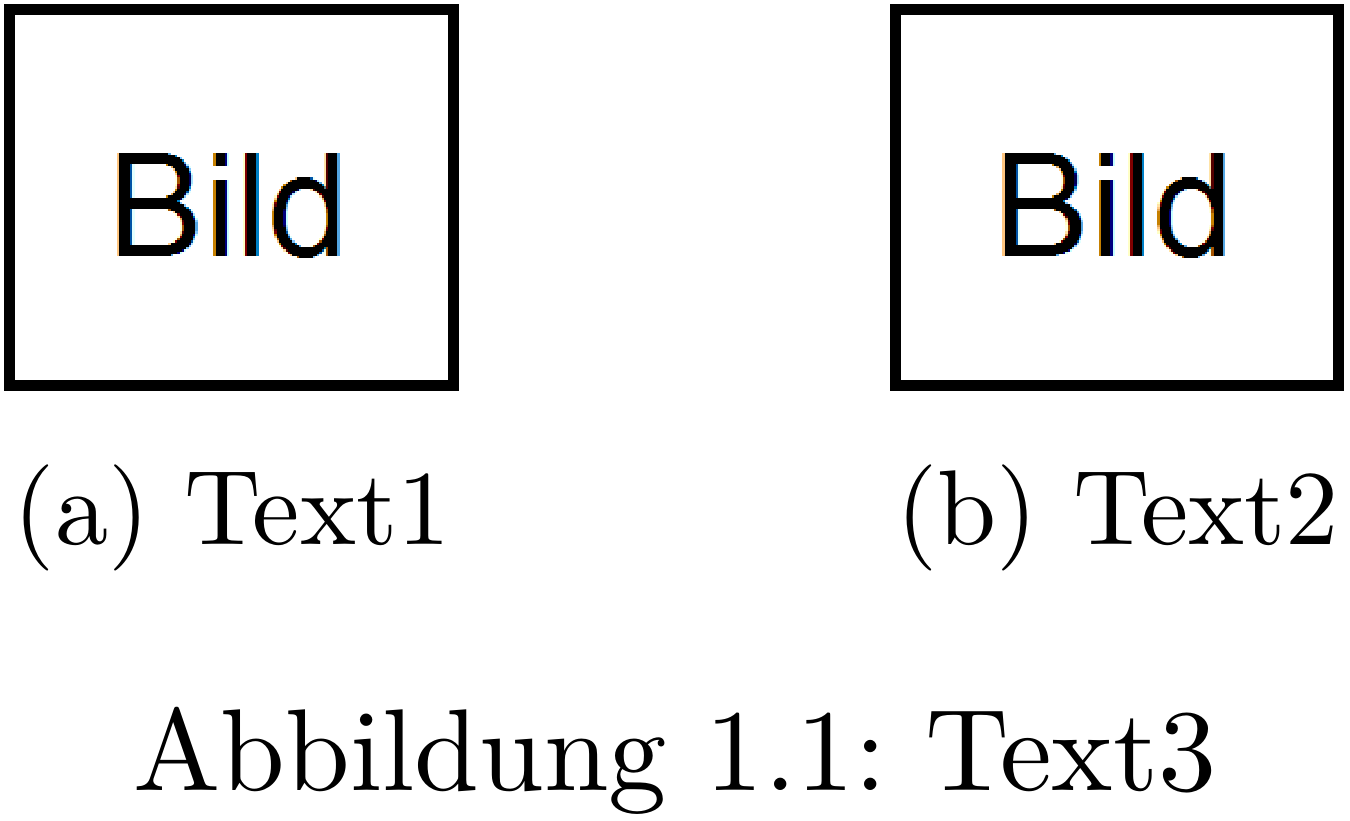
\includegraphics[width=3.5cm,trim={0 7cm 0 0},clip=true]{Bilder/subfigure}
	\captionof{figure}{Text3}
\end{minipage}
%
%
\negAbstand
\begin{lstlisting}
\usepackage{caption,subcaption}
\begin{figure}
\centering
	%
	\begin{subfigure}{0.4\linewidth}
	\centering
		
\includegraphics [width=1.5cm] {Bilder/bild.png}
		\caption{Text1}
	\end{subfigure}
	%
	\begin{subfigure}{0.4\linewidth}
	\centering
		
\includegraphics [width=1.5cm] {Bilder/bild.png}
		\caption{Text2}
	\end{subfigure}
	%
	\caption{Text3}
\end{figure}
\end{lstlisting}



% ----- Eigene Unteschrift -----
\begin{minipage}{\linewidth}
\subsubsectionstageS[3]{Eigene Unterschrift}
%
\begin{minipage}{\linewidth}
		\Centering
	%
	%% Bild Nr. 1
	\begin{minipage}{0.4\linewidth}
		\Centering
    
\includegraphics [width=0.6\linewidth]{Bilder/bild}
		\captionof{figure}{Text}
  \end{minipage}%
	%%
 \hspace{0.1\linewidth}
	%
	%% Bild Nr. 2
  \begin{minipage}{0.4\linewidth}
		\Centering
    
\includegraphics [width=0.6\linewidth]{Bilder/bild}
		\captionof{figure}{Text}
  \end{minipage}
	%
\end{minipage}


% Quellcode:
\vspace{-0.5\baselineskip}
\begin{lstlisting}
\begin{figure}
	\Centering
	\begin{minipage}{0.46\linewidth}
    \Centering
    \includegraphics [width=0.46\linewidth]{Bilder/BILD.png}
		\caption{X}
  \end{minipage}%
	\hspace{1cm}
  %% Bild Nr. 2
  \begin{minipage}{0.46\linewidth}
    \Centering
    \includegraphics [width=0.46\linewidth]{Bilder/BILD.png}
		\caption{X}
  \end{minipage}
\end{figure}
\end{lstlisting}

%%%%%% Quellcode: 
%%%%%\vspace{-0.5\baselineskip}
%%%%%\begin{lstlisting}
%%%%%\begin{figure}{\linewidth}
	%%%%%\Centering
	%%%%%%
	%%%%%\begin{minipage}{0.46\linewidth}
    %%%%%\Centering
    %%%%%\includegraphics [width=1.5cm]{BILD.png}
		%%%%%\captionof{figure}{Bildunterschrift}
  %%%%%\end{minipage}%
  %%%%%%
 %%%%%\hspace{0.5cm}
  %%%%%\begin{minipage}{0.46\linewidth}
    %%%%%\Centering
    %%%%%\includegraphics [width=1.5cm]{BILD.png}
		%%%%%\captionof{figure}{Bildunterschrift}
  %%%%%\end{minipage}
	%%%%%%
%%%%%\end{figure}
%%%%%\end{lstlisting}

\end{minipage}


%%%%%%%%%%%%%%%%%%%%%%%%
\subsectionstage[2]{Textumflossene Bilder}

\begin{multicols}{2}
\begin{wrapfigure}{r}{3cm}
	\centering
	
\includegraphics [width=1cm] {Bilder/bild}
\end{wrapfigure} 
	\bla
%
\columnbreak	
\begin{lstlisting}
\begin{wrapfigure}{r}{3cm}
	\centering
	
\includegraphics [width=1cm] {Bilder/bild.png}
	% \caption[...]{...}
	% \label{fig:...}
\end{wrapfigure} 
\end{lstlisting}
\end{multicols}

\hrule \vspace{0.5\baselineskip}
%----- EOF -----
%%%%%%%%%%%%%%%%%%
\pagebreak
\sectionstage[2]{Listen / Aufzählungen}

%%%%% itemize %%%%%
\begin{multicols}{2}
\begin{itemize} 
	\item TEXT
	\item TEXT
\end{itemize}

\noindent\begin{minipage}{\linewidth}
\begin{lstlisting}
\begin{itemize} 
	\item TEXT
	\item TEXT
\end{itemize}
\end{lstlisting}
\end{minipage}
\end{multicols}

\hrule

%%%%% enumerate %%%%%
\begin{multicols}{2}
\begin{enumerate} 
	\item TEXT
	\item TEXT
\end{enumerate}

\noindent\begin{minipage}{\linewidth}
\begin{lstlisting}
\begin{enumerate} 
	\item TEXT
	\item TEXT
\end{enumerate}
\end{lstlisting}
\end{minipage}
\end{multicols}

\hrule

%%%%% description %%%%%
\begin{multicols}{2}

\begin{description} 
	\item[First] TEXT
	\item[Second] TEXT
\end{description}

\noindent\begin{minipage}{\linewidth}
\begin{lstlisting}
\begin{description} 
	\item[First] TEXT
	\item[Second] TEXT
\end{description}
\end{lstlisting}
\end{minipage}
\end{multicols}

\vspace{-0.5\baselineskip}
\noindent Einzug verändern:\newline
\lstinline|\addtolength{\leftmargini}{-20pt}|

\subsection{Paket \Paket{enumerate}}
Die Nummerierungsart in der Umgebung \Umgebung{enumerate} kann verändert werden.
%%%\negAbstand
\begin{lstlisting}
\usepackage{enumerate}
\begin{enumerate}[(a)]	% Beispiel
	\item ... % (a), (b), (c)
\end{enumerate}
\end{lstlisting}

\subsection{Paket \Paket{enumitem}}
\negAbstand
Alternative  zu \Paket {enumerate}, jedoch mehr Optionen.
Ermöglicht neue Listenumgebungen, die \emph{einfacher anzupassen} sind.



\hrule \vspace{0.5\baselineskip}
%----- EOF -----

%%%%%%%%%%%%%%%%%%
\setlength{\columnseprule}{0.5pt}
\mycolumnbreak

\noindent\begin{minipage}{\linewidth}
\sectionstage[4]{Tabulatoren: Tabbing-Umgebung}

\subsection*{Beispiel}

\begin{tabbing}
ghij \hspace{1em} \=  \kill
a     \> ef \\
ghij \>  klmn
\end{tabbing}

\vspace{-0.5\baselineskip}
\begin{lstlisting}
\begin{tabbing}
	ghij \hspace{1em} \=  		\kill
	a                 \> ef 	\\
	ghij              \> klmn
\end{tabbing}
\end{lstlisting}

\end{minipage}

Hinweis: Innerhalb der Tabbing-Umgebung gibt es keinen automatischen Zeilenumbruch!

%%%%%%%%%%%%%%%%%%%%%%%%
\subsection*{Musterzeile}
\vspace{-0.5\baselineskip}
\begin{lstlisting}
\=			% Tabulator für Musterzeile
\kill		% Zeilenende. Zeile wird nicht ausgegeben
\end{lstlisting}

%%%%%%%%%%%%%%%%%%%%%%%%
\subsection*{Normale Zeilen}
\vspace{-0.5\baselineskip}
\begin{lstlisting}
\\ 			% Zeilenende
\>			% zum nächsten Tabulator
\<			% zum vorhergehenden Tabulator
a \` b	% a links, b rechts vom Tabulator
\end{lstlisting}
%
\hrule \vspace{0.5\baselineskip}
%----- EOF -----
%%%%%%%%%%%%%%%%%%%
\columnbreak
\sectionstage[2]{Tabellen}
%
\noindent\begin{minipage}{\linewidth}
	%\captionof{table}{TEXT}
	\Centering
	\begin{tabular}{|l|r c l|}
		\hline
			1 &rechts	& mittig& links\\
			2 &a 			& b 		& c \\
		\cline{2-4}
			3 &\multicolumn{3}{c|}{mehrere Spalten}\\
		\hline
	\end{tabular}
\end{minipage}

\begin{lstlisting}
\begin{table}
	\caption{TABELLENÜBERSCHRIFT}
	\label{KEY}
	\centering
	\begin{tabular}{|l|r c l|}
		\hline
			1 &rechts& mittig& links\\
			2 &a & b & c \\
		\cline{2-4}
			3 &\multicolumn{3}{c|}{mehrere Spalten}\\
		\hline
	\end{tabular}
\end{table}
\end{lstlisting}
%
%%%%%%%%%%%%%%%%%%%%%
\subsectionstage[3]{Schönere Tab. (\Paket{booktabs})}

\noindent\begin{minipage}{\linewidth}
\Centering
\begin{tabular}{cc}
\toprule
Spalte 1 & Spalte 2 \\
\midrule
eins & zwei\\
drei & vier\\
\bottomrule
\end{tabular}
\end{minipage}
%
%\begin{minipage}{0.5\linewidth}
\begin{lstlisting}
\usepackage{booktabs}
\begin{tabular}{cc}
	\toprule
		Spalte 1 & Spalte 2 \\
	\midrule
		eins & zwei\\
		drei & vier\\
	\bottomrule
\end{tabular}
\end{lstlisting}
%\end{minipage}


\vspace{-1\baselineskip}
\subsubsection*{Befehls-Übersicht}
\negAbstand

\begin{lstlisting}
\toprule[LEN](			% LEN: Liniendicke
\midrule[LEN]
\bottomrule[LEN]
\cmidrule[LEN](TRIM){A-B}	% Zusätzliche Linie zwischen den Spalten A und B. TRIM: r, r{LEN}, l oder l{LEN}
\addlinespace[LEN]	% Zusätzlicher Zeilenabstand
\end{lstlisting}

\Paket{booktabs} ist kombinierbar mit den Umgebungen \Umgebung{tabular}, \Umgebung{array}(\verb|\usepackage{array}|) und \Umgebung{longtable} (\verb|\usepackage{longtable}|).

%%%%%%%%%%%%%%%%%%%%%
%\columnbreak
\subsectionstage[2]{Feste Tab.-breite (\Paket{tabularx})}
Beispiel (noch näher erläutern!):
\begin{lstlisting}
\usepackage{tabularx}
	\newcolumntype{L}[1]{>{\RaggedRight \arraybackslash}p{#1}} % linksbündig	%mit tabularx neue Spaltentypen definieren.
	\newcolumntype{M}[1]{>{\RaggedRight \arraybackslash}m{#1}} % linksbündig
	
	\newcolumntype{C}[1]{>{\Centering \arraybackslash}p{#1}} % zentriert
	\newcolumntype{D}[1]{>{\Centering \arraybackslash}m{#1}} % zentriert
		
	\newcolumntype{R}[1]{>{\RaggedLeft \arraybackslash}p{#1}} % rechtsbündig
	
	\newcolumntype{B}[1]{>{\arraybackslash}p{#1}}	%Blocksatz
\end{lstlisting}

\negAbstand

%%%%%%%%%%%%%%%%%%%%%
\subsectionstage[4]{Farbige Tab. (\Paket{colortbl})}
\negAbstand
\begin{lstlisting}
\usepackage{array,color} % oder xcolor
\usepackage{colortbl}
\end{lstlisting}

\negAbstand\negAbstand

%%%%%
\begin{multicols}{2}
%
\begin{lstlisting}
\arrayrulecolor{red}		% Farbe der Tabellen-Linien

\begin{tabular}{|
	>{\columncolor{lime}}l|
	>{\columncolor{lightgray}}c|
	}
	\toprule %o.\hline
		eins & zwei\\
		drei & vier\\
	\bottomrule
\end{tabular}
\end{lstlisting}

\arrayrulecolor{red}		% Farbe der Tabellen-Linien
\begin{tabular}{|
	>{\columncolor{lime}}l|
	>{\columncolor{lightgray}}c|
	}
\toprule
eins & zwei\\
drei & vier\\
\bottomrule
\end{tabular}

\columnbreak

\begin{lstlisting}
\begin{tabular}{lc}
	\rowcolor{Goldenrod}
	eins 
	& zwei\\
	drei 
	& \cellcolor{Tan} vier\\
\end{tabular}
\end{lstlisting}

\arrayrulecolor{black}
\begin{tabular}{lc}
\toprule
\rowcolor{Goldenrod}eins & zwei\\
drei & \cellcolor{Tan}vier\\
\bottomrule
\end{tabular}


\end{multicols}
%%%%%

%%%%%%%%%%%%%%%%%%%%%
\subsectionstage[3]{Mehrseitige Tab. (\Paket{longtable})\hspace{-0.8ex}}
Benutzbar wie die \Umgebung{tabular}-Umgebung.

%\begin{multicols}{2}
\begin{lstlisting}
\usepackage{longtable}
\usepackage{booktabs}		% in diesem Beispiel verwendet

\begin{longtable}{c|c|c|}
	\caption{Nährstofftabelle}\\
	% % Kopfzeile der ersten Seite
	\toprule
	...
	\\ \midrule \endfirsthead 
	%% Kopfzeile ab der zweiten Seite
	\toprule
	...
	\\ \midrule \endhead
	% % Fußzeile der ersten Seite
	...
	\bottomrule	\endfoot
	%% Fußzeile ab der zweiten Seite
	...
	\bottomrule \endlastfoot
	<Inhalt der Tabelle>
\end{longtable}
\end{lstlisting}
%\end{multicols}
\negAbstand


%%%%%%%%%%%%%%%%%%%%%
\subsectionstage[2]{Doppelte Linien in Tabellen (\Paket{hhline})}
%\negAbstand


\noindent\begin{minipage}{\linewidth}
\Centering
\begin{tabular}{||cc||c|c||} \hhline{|t:==:t:==:t|}
a & b & c & d \\ \hhline{|:==:|~|~||}
w & x & y & z \\ \hhline{|b:==:b:==:b|}
\end{tabular}
\end{minipage}
%
%\noindent\begin{minipage}{0.5\linewidth}
\begin{lstlisting}
\begin{tabular}{||cc||c|c||} \hhline{|t:==:t:==:t|}
a & b & c & d \\ \hhline{|:==:|~|~||}
w & x & y & z \\ \hhline{|b:==:b:==:b|}
\end{tabular}
\end{lstlisting}
%\end{minipage}
%
\hrule
%
\posAbstand

\noindent\begin{minipage}{\linewidth}
\Centering
\begin{tabular}{||cc||c|c||} \hhline{|t:==:t:==:t|}
a & b & c & d \\\hhline{|:==:|~|~||}
1 & 2 & 3 & 4 \\\hhline{#==#~|=#}
i & j & k & l \\\hhline{||--||--||}
w & x & y & z \\\hhline{|b:==:b:==:b|}
\end{tabular}
\end{minipage}
%
%\begin{minipage}{0.5\linewidth}
\begin{lstlisting}
\begin{tabular}{||cc||c|c||} \hhline{|t:==:t:==:t|}
a & b & c & d \\ \hhline{|:==:|~|~||}
1 & 2 & 3 & 4 \\ \hhline{#==#~|=#}
i & j & k & l \\ \hhline{||--||--||}
w & x & y & z \\ \hhline{|b:==:b:==:b|}
\end{tabular}
\end{lstlisting}
%\end{minipage}
%


\negAbstand

%%%%%%%%%%%%%%%%%%%%%
\subsectionstage[1]{Tabellenformat anpassen}
\negAbstand
\begin{lstlisting}
\setlength{\extrarowheight}{4pt} % extra Zeilenhöhe (Tabellenzeilen) 
\renewcommand{\arraystretch}{Faktor}	% Abstand zwischen Zeilen ändern. (Textzeilen) oder \setstretch{Faktor} (Paket setspace)
\setlength{\tabcolsep}{6pt}		% Abstand zwischen Spalten ändern
\end{lstlisting}
\negAbstand
\hrule \vspace{0.5\baselineskip}
%----- EOF -----
%%%%%%%%%%%%%%%%%%%
\setlength{\columnseprule}{0.5pt}
%\mycolumnbreak
\pagebreak

\sectionstage[2]{Mathematik}\label{cha:mathe}
\todo{Wo werden welche Pakete benötigt?}

\subsectionstage[3]{Umgebung für Mathe im Fließtext}
\begin{tabular}{c|c}
\lstinline|\begin{math} a=3 \end{math}| &  \begin{math} a=3 \end{math} \\

\lstinline|$ a=3 $| 			&  $ a=3 $ \\
\end{tabular}


%\subsectionstage[2]{Häufige Zeichen und Operatoren}


\setlength{\columnseprule}{0.5pt}
\subsection{Wichtige Operatoren}
%\begin{multicols}{2}
\begin{tabbing}
$\lim_{x\to 0}$ \hspace{2em}	\= 	\kill

$\frac{2}{3}$			\>	\lstinline|\frac{2}{3}|	\\
$\sqrt{2}$				\> 	\lstinline|\sqrt{2}|		\\
$\sqrt[3]{2}$			\> 	\lstinline|\sqrt[3]{2}|	\\
$\int \limits_{0}^{1}$			\> 	\lstinline|\int\limits_{0}^{1}|	\\
$\int\nolimits_{0}^{1}$		\> 	\lstinline|\int\nolimits_{0}^{1}|	\\
$\int_{0}^{1}$		\> 	\lstinline|\int_{0}^{1}|	\\

$\int\!\!\!\int_{D} \mathrm{d}x\,\mathrm{d}y$		
	\> 	\lstinline|\int\!\!\!\int_{D}| 	\\
	\> \lstinline|\mathrm{d}x \,| \\
	\> \lstinline|\mathrm{d}y|	\\
	
$\lim_{x\to 0}$		\> 	\lstinline|\lim_{x\to 0}|	\\
$x' x''$						\> \lstinline|x' x''| \\
$x^{a+b}$		\> 	\lstinline|x^{a+b}|	\\
$x_{a1}$		\> 	\lstinline|x_{a1}|	\\

$\hat x$							\> 	\lstinline|\hat x|	\\
$\tilde x$						\> 	\lstinline|\tilde x|	\\
$\widehat{xyz}$				\> 	\lstinline|\widehat{xyz}|	\\
$\widetilde {xyz}$		\> 	\lstinline|\widetilde {xyz}|	\\
$\overline x$					\> 	\lstinline|\overline x|	\\
$\underline x$				\> 	\lstinline|\underline x|	\\
$\vec x$							\>  \lstinline|\vec x| \\
$\overbrace{1+2}^{x}$		\> 	\lstinline|\overbrace{1+2}^{x}|	\\
$\underbrace{1+2}_{x}$		\> 	\lstinline|\underbrace{1+2}_{x}|	\\
%$n\choose k$		\> 	\lstinline|{n\choose k}|	\\[1ex]
%${x\atop y}$		\> 	\lstinline|{x\atop y}| \\[1ex]
$\overset{B}{A}$		\> 	\lstinline|\overset{B}{A}|	\\[1ex]
$\underset{B}{A}$		\> 	\lstinline|\underset{B}{A}| \\[1ex]
${\binom{a}{b}}$		\> 	\lstinline|\binom{a}{b}|
\end{tabbing}

%\end{multicols}

%%%%%%%%%%
%\genfrac{l}{r}{w}{s}{zähler}{nenner}
%genfrac dient der flexiblen Erzeugung von Brüchen. Dabei steht
    %l für einen optionalen linken Begrenzer (z.B. [),
    %r für einen optionalen rechten Begrenzer (z.B. ]),
    %w für die Dicke des Bruchstriches (width). Default ist 1pt,
    %s für den Style. Default ist 1. Gültige Werte sind 0,1,2,3 für \displaystyle, \textstyle, \scriptstyle, \scriptscriptstyle
		%%%%%%%%%%
\setlength{\columnseprule}{0.5pt}


\begin{multicols}{4}
\begin{lstlisting}
\sin
\cos
\tan
\cot
\arccos
\arcsin
\arctan
\sinh
\cosh
\tanh
\coth

\exp
\ln
\lg
\log

\min
\max 

\arg
\csc
\deg 
\det 
\dim
\gcd
\hom
\inf
\ker
\lim
\liminf
\limsup
\pmod
\Pr
\sec
\sup 
\end{lstlisting}

\end{multicols}


\subsubsection*{Paket \Paket{nicefrac}}
\lstinline|\nicefrac{2}{3}|: 
	\hspace{1em} \nicefrac{2}{3} 
	\hspace{1em} (auch außerhalb Mathe-Umgebung)

% ----- Matrizen ----- ------ -----
\subsectionstage[3]{Matrizen und Vektoren}
% ---- Matrix ----
\begin{minipage}{0.3\linewidth}
$\begin{matrix} 1 & 2 \\ 3 & 4 \end{matrix}$
\end{minipage}
%
\begin{minipage}{0.5\linewidth}
\begin{lstlisting}
\begin{matrix}
	 1 & 2 \\ 3 & 4 
\end{matrix}
\end{lstlisting}
\end{minipage}
%%%%%
\negAbstand
\begin{minipage}{0.3\linewidth}
$\begin{smallmatrix} 1 & 2 \\ 3 & 4 \end{smallmatrix}$
\end{minipage}
%
\begin{minipage}{0.5\linewidth}
\begin{lstlisting}
\begin{smallmatrix}
	 1 & 2 \\ 3 & 4
\end{smallmatrix}
\end{lstlisting}
\end{minipage}
%%%%%
\negAbstand
% ----- pmatrix -----
\begin{minipage}{0.3\linewidth}
$\begin{pmatrix} 1 & 2 \\ 3 & 4 \end{pmatrix}$
\end{minipage}
%
\begin{minipage}{0.5\linewidth}
\begin{lstlisting}
\begin{pmatrix}
	 1 & 2 \\ 3 & 4 
\end{pmatrix}
\end{lstlisting}
\end{minipage}
%%%%%
%
\verb|vmatrix:| $\begin{vmatrix} 1 \end{vmatrix}$
\qquad
\verb|Vmatrix:| $\begin{Vmatrix} 1 \end{Vmatrix}$
\qquad
\verb|bmatrix:| $\begin{bmatrix} 1 \end{bmatrix}$
\qquad
\verb|Bmatrix:| $\begin{Bmatrix} 1 \end{Bmatrix}$
%
% ----- cases -----
\begin{minipage}{0.3\linewidth}
$\begin{cases}
	%a & \text{für} & x \geq 3 \\
	%a & \text{für} & x < 3
	1 & 2 \\ 3 & 4
\end{cases}$
\end{minipage}
%
\begin{minipage}{0.5\linewidth}
\begin{lstlisting}
\begin{cases}
	 1 & 2 \\ 3 & 4 
\end{cases}
\end{lstlisting}
\end{minipage}
%
% ----- Array -----
\negAbstand
\begin{minipage}{0.3\linewidth}
$\begin{array}{cc} 1 & 2 \\ 3 & 4 \end{array}$ 
\end{minipage}
\begin{minipage}{0.5\linewidth}
\begin{lstlisting}
\begin{array}{cc}
		1 & 2 \\ 3 & 4
\end{array}
\end{lstlisting}
\end{minipage}
%%%%%


%%%%%%%%%%%%
\subsectionstage[3]{Formatierungen}
\setlength{\columnseprule}{0.5pt}
\begin{tabbing}
	$\mathbf{ABCabc}$		\= \lstinline|\mathnormal{ABCabc}| \=		\kill
	%
	$\mathnormal{ABCabc}$	\> \lstinline|\mathnormal{ABCabc}|	 \small default
	\\
	$\mathrm{ABCabc}$		\> \lstinline|\mathrm{ABCabc}|	\> \small roman
	\\
	$\mathbf{ABCabc}$		\> \lstinline|\mathbf{ABCabc}|	\> \small bold roman
	\\
	$\mathsf{ABCabc}$		\> \lstinline|\mathsf{ABCabc}|	\> \small sans serif
	\\
	$\mathit{ABCabc}$		\> \lstinline|\mathit{ABCabc}|	\> \small text italic
	\\
	$\mathtt{ABCabc}$		\> \lstinline|\mathtt{ABCabc}|	\> \small typewriter
	\\
	$\mathcal{ABCabc}$	\> \lstinline|\mathcal{ABCabc}|	\> \small calligraphic
	\\
	$\mathbb{RQZNPC}$	\> \lstinline|\mathbb{RQZNP}| 
		{\footnotesize\slshape(\Paket{amssymb})}
	\\[0.5\baselineskip]
	%

\textbf{Schriftgrößen:} 
	\\
	$\displaystyle Text$ \> \lstinline|\displaystyle Text|
		\\
	$\textstyle Text$ \> \lstinline|\textstyle Text|
		\\
	$\scriptstyle Text$ \> \lstinline|\scriptstyle Text|
		\\
	$\scriptscriptstyle Text$ \> \lstinline|\scriptscriptstyle Text|
\end{tabbing}


\subsectionstage[3]{Klammern}
\begin{tabbing}
\hspace{2.5em} \=  \hspace{3em} 
\= \hspace{2.5em} \= \hspace{3em}
\= \hspace{2.5em} \= \hspace{3em} \kill
$( \dots)$								\> \lstinline|()|	\>
$[ \dots]$								\> \lstinline|[]|	\>
$\{ \dots\}$							\> \lstinline|\{ \}	|	\\
$\lbrace \dots\rbrace$		\> \lstinline|\lbrace \rbrace|	\\
$\langle \dots\rangle$		\> \lstinline|\langle \rangle|	
\end{tabbing}
%\negAbstand
%
\begin{tabbing}
$(\frac{a}{b})$ \hspace{1ex}  \= \lstinline|(\frac{a}{b})|  \\

$\left(\frac{a}{b}\right)$  
	\> \lstinline|\left(\frac{a}{b}\right) % autom. Größe|  \\
	
$\bigl(\frac{a}{b}\bigr)$  
	\> \lstinline|\bigl(\frac{a}{b}\bigr)|  \\
	
$\Bigl(\frac{a}{b}\Bigr)$  
	\> \lstinline|\Bigl(\frac{a}{b}\Bigr)|  \\
	
$\biggl(\frac{a}{b}\biggr)$  
	\>	\begin{minipage}{0.6\linewidth}
				\lstinline|\biggl(\frac{a}{b}| 
				\lstinline|\biggr)|
			\end{minipage} \\
	
$\Biggl(\frac{a}{b}\Biggr)$  
	\> \begin{minipage}{0.6\linewidth}
				\lstinline|\Biggl(\frac{a}{b}|
				\lstinline|\Biggr)|  
			\end{minipage} \\
	
\end{tabbing}
%\ifaklein{}{
	%\end{multicols}
%}

\negAbstand
\subsectionstage[2]{Umgebungen für Mathe in separater Zeile}

\addtolength{\leftmargini}{-15pt}
\begin{itemize}
	\item {\bfseries equation oder \lstinline|\[ \]|}: Einzelne abgesetzte Gleichung
	\item multline: (Einzelne) Gleichung über mehrere Zeilen
	\item gather: 	Mehrere Gleichungen
	\item {\bfseries align}: 		Mehrere Gleichungen mit Ausrichtungspunkten
	\item flalign: 	wie align, jedoch rechts-/links-bündig
	\item *: jeweils ohne Gleichungs-Nummerierung (\mbox{\bfseries equation*}, 
	multline*, 
	gather*, 
	{\bfseries align*}, 
	flalgin*)
\end{itemize}
\addtolength{\leftmargini}{15pt}

\setlength{\columnseprule}{0.5pt } % Trennlinie für multicols


\newcommand{\myhruleB}{
	\myhrule\negAbstand
	}

%%%%% \[ \] %%%%%
\begin{multicols}{2}
\begin{lstlisting}
\[
	ab = c
\]
\end{lstlisting}
\columnbreak \hspace{0.5\baselineskip}
\[
	ab = c
\]
\end{multicols}

\myhruleB

%%%%% equation %%%%%
\begin{multicols}{2}
\begin{lstlisting}
\begin{equation} 
	ab = c \\
	d	 = ef
\end{equation}
\end{lstlisting}
\columnbreak
\begin{equation} 
	ab = c 
\end{equation}
\end{multicols}


\myhruleB

%%%%% multline %%%%%
\begin{multicols}{2}
\begin{lstlisting}
\begin{multline} 
	ab = c \\
	d	 = ef
\end{multline}
\end{lstlisting}
\begin{multline} 
	ab = c \\
	+ d \cdot ef
\end{multline}
\end{multicols}

\myhruleB

%%%%% gather %%%%%
\begin{multicols}{2}
\begin{lstlisting}
\begin{gather} 
	ab = c \\
	d	 = ef
\end{gather}
\end{lstlisting}
\begin{gather} 
	ab = c \\
	d	 = ef
\end{gather}
\end{multicols}

\myhruleB

%%%%% align %%%%%
\begin{multicols}{2}
\begin{lstlisting}
\begin{align} 
	ab&=c 	& d	&= ef \\
	g &=hi 	& j &= k 
\end{align}
\end{lstlisting}
\begin{align} 
	ab&=c 	& d	&= ef \\
	g &=hi 	& j &= k 
\end{align}
\end{multicols}

\myhruleB

%%%%% flalign %%%%%
\begin{multicols}{2}
\begin{lstlisting}
\begin{flalign} 
	ab&=c 	& d	&= ef \\
	g &=hi 	& j &= k 
\end{flalign}
\end{lstlisting}
\columnbreak
\begin{flalign} 
	ab&=c 	& d	&= ef \\
	g &=hi 	& j &= k 
\end{flalign}
\end{multicols}

\subsubsection*{Gleichungsnummer verändern}
\negAbstand\negAbstand
\begin{multicols}{2}
\begin{lstlisting}
\begin{align} 
	ab&=c  \tag{$*$} 	\\
	ab&=c  \notag 		\\
	ab&=c
\end{align}
\end{lstlisting}
\begin{align} 
	ab&=c  \tag{$*$} 	\\
	ab&=c  \notag 		\\
	ab&=c 
\end{align}
\end{multicols}

\begin{equation}
%\numbereq
	a = b
	%\label{eq:}
\end{equation}


\noindent \begin{minipage}{\linewidth}
\subsectionstage[1]{Erweiterte Formatierungen}
\negAbstand
\begin{lstlisting}
\usepackage[OPTIONEN]{amsmath}		% Erweiterter Mathematiksatz
	% Option leqno:  Gleichungsnummer links
	% Option requno: Gleichungsnummer rechts
	% Option fleqn:  Formel mit Einzug. Einzug in Präambel definierbar mit: \setlength\mathindent{5mm}
	
% Abstände Matheumgebungen
\setlength\abovedisplayshortskip{0pt}		% ?
\setlength\belowdisplayshortskip{10pt}	% ?
\setlength\abovedisplayskip{0pt}				% kein Abstand vor Gleichungsumgebungen
\setlength\belowdisplayskip{20pt}				% ?
\end{lstlisting}

\subsubsection*{Mathe in Überschriften \stage{1}}
Schriftart anpassen (nur KOMA-Klassen):
\begin{lstlisting}
	\renewcommand*{\sectfont}{\sffamily\bfseries\boldmath}
\end{lstlisting}

\end{minipage}


\hrule \vspace{0.5\baselineskip}
%----- EOF -----



\mycolumnbreak
\sectionstage[2]{Zeichnen (Paket \Paket{tikz})}
Quelle:	\url{http://www.tn-home.de/TUGDD/Stuff/TikZ_final.pdf}

Hinweis vorweg: Man sollte sich gut überlegen, ob man wirklich innerhalb von LaTeX zeichnen möchte, oder ob ein Zeichenprogramm wie z.B. Inkscape besser geeignet ist.


\subsection{Basics}
\begin{lstlisting}
\usepackage{tikz} % läd intern auch das Paket pgf
\usetikzlibrary{arrows,automata,backgrounds,calendar} % bei Bedarf
??? \tikzoptions ???????	

\draw(0,0) -- (2,2); 			 %Linie
\draw[->](0,0) -- (2,2);	%Pfeil
\draw[step=0.1,gray,very thin] (0,0) grid (1,1);		% Gitter zeichnen
\draw[OPT,OPT]  ....
\end{lstlisting}

\subsubsection{OPTionen}
\begin{lstlisting}
%Pfeilsorten:
->
<-
|-> 
<-> 
>->>

%Linienstärken:
ultra thin
very thin
thin
semithick
thick
very thick
ultra thick
(help lines)
line width=12
line width=0.2cm

%Linien-Eigenschaften:
dashed
dottet
rounded corners 	%(runde Ecken)
red			(Farben: red, green, blue, cyan, magenta, yellow, black, gray, darkgray, ligthgray, brown, olive, orange, pink, purple, teal, violet, white.)	\\

%Farben:
\node[...,fill=black!60!green,...]
\node[...,fill={rgb:red,4;green,2;yellow,1},...]
% in LaTeX selbst definierte Farben können auch verwendet werden.
\end{lstlisting}

\subsubsection{Koordinaten}
\begin{lstlisting}
\draw[->] (0,0) -- (2, 2);			% absoulte Koordinaten
\draw[->] (2,0) -- +(2, 2);			% relative Koordinaten mit "+", unveränderter Referenzpunkt
\draw[->] (2,0) -- ++(2, 2);			% relative Koordinaten mit "++", veränderter Referenzpunkt
\draw (0:1cm) -- (72:1cm) -- (2*72:1cm)	% Polarkoordinaten mit (winkel:radius)
\end{lstlisting}

% ----- ----- -----------------------------
\subsection{Objekte zeichnen}
\lstinline|\begin{tikzpicture}	...	\end{tikzpicture}|

\subsubsection{Kurven zeichnen}
(\url{http://www.math.tugraz.at/~huss/new/teaching/computermathematik09/dateien/tikz_demonstration.pdf})
\begin{lstlisting}
\draw (0,0) .. controls (0,1) and (1,1) .. (2, 2);	% Direkte Eingabe der Kontrollpunkte
\draw[bend left=30] (3,0) to (4, 2);		% Die Line krümmt sich um 30 Grad nach Links
\draw[out=90, in=-90] (6,0) to (7, 2);		% aus- und eingehenden Winkel festlegen
\end{lstlisting}

\subsubsection{Ellipsen und Kreise}
\begin{lstlisting}
\draw (0,0) circle (10pt);		% Kreis
\draw (2,0) ellipse (10pt and 5pt);
\end{lstlisting}

\subsubsection{Objekte füllen}
\begin{lstlisting}
\fill (0,0) circle (0.25);
\fill[red] (1,0) circle (0.25);
\fill[blue] (2,0) circle (0.25);
\shade[ball color=green] (3,0) circle (0.25);
\fill[orange] (4,0) circle (0.25);
\fill[green,opacity=0.5] (4.25,0) circle (0.25);
\end{lstlisting}





%-------------------------------------
\columnbreak


\subsection*{Beispiel}

\begin{minipage}{0.34\linewidth}
	\begin{tikzpicture}[scale=0.4]
		\tikz 
		\draw[thick,rounded corners=8pt] (0,0) -- (0,2) -- (1,3.25) -- (2,2) -- (2,0) -- (0,2) -- (2,2) -- (0,0) -- (2,0);
	\end{tikzpicture}
\end{minipage}
%
%
\begin{minipage}{0.69\linewidth}
\begin{lstlisting}
\begin{tikzpicture}[scale=0.4]
	\tikz \draw[thick,rounded corners=8pt] (0,0) -- (0,2) -- (1,3.25) -- (2,2) -- (2,0) -- (0,2) -- (2,2) -- (0,0) -- (2,0);
\end{tikzpicture}
\end{lstlisting}
\end{minipage}

\usetikzlibrary{circuits.ee.IEC}
\begin{tikzpicture}[circuit ee IEC]
	\draw (0,0) to [resistor] (2,0) to [inductor] (4,0);
\end{tikzpicture}

\bigskip

%\begin{tikzpicture}[
	%circuit ee IEC,
	%x=3cm,y=2cm,
	%semithick,	
	%every info/.style={font=\footnotesize},	
	%small circuit symbols,	
	%set resistor graphic=var resistor IEC graphic,	
	%set diode graphic=var diode IEC graphic,	
	%set make contact graphic= var make contact IEC graphic]
	%
	%% Let us start with some contacts:
	%\foreach \contact/\y in {1/1,2/2,3/3.5}
	%{
		%\node [contact] (left contact \contact) at (0,\y) {};
		%\node [contact] (right contact \contact) at (1,\y) {};
	%}
	%
	%%\foreach \contact/\y in {1/1,2/2,3/3.5,4/4.5,5/5.5}
	%%{
		%%\node [contact] (left contact \contact) at (0,\y) {};
		%%\node [contact] (right contact \contact) at (1,\y) {};
	%%}
	%%\draw (right contact 1) -- (right contact 2) -- (right contact 3)
	   %%-- (right contact 4) -- (right contact 5);
	%%\draw (left contact 1) to [diode] ++(down:1)
		%%to [voltage source={near start,
												%%direction info={volt=3}},
				%%resistor={near end,ohm=3}] ++(right:1)
		%%to (right contact 1);
	%%\draw (left contact 1) to [resistor={ohm=4}] (right contact 1);
	%%\draw (left contact 1) to [resistor={ohm=3}] (left contact 2);
	%%\draw (left contact 2) to [voltage source={near start,
																%%direction info={<-,volt=8}},
											%%resistor={ohm=2,near end}] (right contact 2);
	%%\draw (left contact 2) to [resistor={near start,ohm=1},
														%%make contact={near end,info'={[red]$S_1$}}]
											%%(left contact 3);
	%%\draw (left contact 3) to [current direction'={near start,info=$\iota$},
		%%resistor={near end,info={$R=4\Omega$}}]
		%%(right contact 3);
	%%\draw (left contact 4) to [voltage source={near start, direction info={<-,volt=8}}, 		resistor={ohm=2,near end}] (right contact 4);
	%%\draw (left contact 3) to [resistor={ohm=1}] (left contact 4);
	%%\draw (left contact 4) to [resistor={ohm=3}] (left contact 5);
	%%\draw (left contact 5) to [resistor={ohm=4}] (right contact 5);
	%%\draw (left contact 5) to [diode] ++(up:1)
		%%to [voltage source={near start,
		%%direction info={volt=3}},
		%%resistor={near end,ohm=3}] ++(right:1)
		%%to (right contact 5);
%\end{tikzpicture}

%%%%%%%%%%%%%%%%%%%%%%%%%%

\sectionstage[0]{Plotten}
\lstinline|\usepackage{pgfplots}|\\
siehe \url{http://www.golatex.de/wiki/Diagramme_mit_LaTeX}\\

\noindent
\lstinline|\usepackage{filecontents}|

scale, xscale, yscale

%\begin{tikzpicture}
	%\addplot gnuplot 
  %[id=exp,mark=none,domain=0:8, very thick]{x**2+10}; 
 %\addplot gnuplot
   %[raw gnuplot,id=bal,mark=none,very thick]{
    %set xrange  [0:10];
    %f(x)=a*x+b;
    %fit f(x) "data.dat" via a,b;
    %plot f(x)};
 %\addplot plot
  %[only marks,mark=x,thick] 
  %file {data.dat};
%\end{axis} 
%\end{tikzpicture} 

\hrule \vspace{0.5\baselineskip}
%----- EOF -----
%\columnbreak
\mycolumnbreak


\sectionstage[2]{Quelltexte}
\subsectionstage[4]{verbatim-Umgebung}
\negAbstand
\begin{lstlisting}
	\verb|Direkt ausgegebener Text|
	\begin{verbatim}
		Direkt ausgegebener Text
	\end{verbatim}
\end{lstlisting}
\Befehl{verb} und \Umgebung{verbatim} können nicht als Paramter an andere Befehle übergeben werden.

\subsectionstage[2]{Quelltext (Paket \Paket{listings})}

siehe auch: \url{http://en.wikibooks.org/wiki/LaTeX/Source_Code_Listings}

Für escape-Inside-Option hier nachschlagen: \url{http://tex.stackexchange.com/questions/110268/texcl-escapeinside-and-single-character-comments-with-listings-package}

\subsubsection*{Umlaute bei utf8-Codierung}
{\footnotesize
Bei Verwendung der Kodierung utf8 (\lstinline|\usepackage[utf8]{inputenc}|) können Umlaute (ä ö ü ß) nicht ohne weiteres  dargestellt werden. Abhilfe (Quelle \url{http://uweziegenhagen.de/?p=1500}; \qquad\qquad\qquad 2014):
}
%
\begin{lstlisting}
\lstset{literate=%
    {Ö}{{\"O}}1
    {Ä}{{\"A}}1
    {Ü}{{\"U}}1
    {ß}{{\ss}}1
    {ü}{{\"u}}1
    {ä}{{\"a}}1
    {ö}{{\"o}}1
    %{~}{{\textasciitilde}}1
}
 %ODER:
\lstset{texcl=true} % Schriftsatz mit LaTeX. (Unter Umständen unerwünscht.)
\end{lstlisting}

%\columnbreak
\subsubsection{\Paket{listings}: Einstellungen}
\negAbstand
\lstset{mathescape = true}

\begin{lstlisting}
\usepackage{listings}
\lstset{
		language		=	[LaTeX]{TeX},		%[dialect]{language}
		% Mögliche Sprachen (Auswahl): Assembler, Basic, C++, Delphi, Fortran, Gnuplot, HTML, Java, Mathematica, Matlab, Octave, Perl, PHP, Python, Scilab, SQL, TeX, [LaTeX]{TeX}, VHDL, XML
		%escapeinside = {((**} {**xx},		% ???
		% escapebegin = {((**} 						% ???
		% escapeend		= {**))}						% ???
\end{lstlisting}
\vspace{-1\baselineskip}
\begin{lstlisting}
		basicstyle	=	\ttfamily,
		basicstyle	=	\small,
		identifierstyle=\ttfamily,
		commentstyle=	\ttfamily,
		commentstyle=	\color{gray},
		stringstyle =	\ttfamily,
		keywordstyle=	\ttfamily,
		keywordstyle=	\color{OliveGreen},
\end{lstlisting}
\vspace{-1\baselineskip}
\begin{lstlisting}
		numbers			=	left,  			% (none, left, right)
		numberstyle	=	\tiny, 			
		stepnumber	=	1,    			% Step between two line-numbers
		numbersep		=	5pt,  			% How far are line-numbers from code
		backgroundcolor=\color{white},		
		frame				=	none,       % A frame around the code
		tabsize			=	2,					% Default tab size
		captionpos	=	b,          % Caption-position = bottom
\end{lstlisting}

\vspace{-1\baselineskip}
\begin{lstlisting}
		breaklines	=	true,       % Automatic line breaking?
		breakatwhitespace=false,  % Automatic breaks only at whitespace?
		showspaces	=	false,      % Dont make spaces visible
		showstringspaces = false	% Leerzeichen in Strings anzeigen
		showtabs		=	false,      % Dont make tabls visible
		columns			=	fixed, 			% Column format  (flexible, fixed or fullflexible)
		% morekeywords   = {Wort3, Wort4}
		% deletekeywords = {Wort1, Wort2}

\end{lstlisting}
\vspace{-1\baselineskip}
\begin{lstlisting}
	%	% Escape to LaTeX:
	%	mathescape = true, 	% $a=x$ Mathemodus ermöglichen
		escapechar = {$^2$},		% Buchstabe zum Verlassen und Zurückkehren (LaTeX-Modus)
	% escapeinside={$^2$}{$^2$},	% Alternative zu escapechar
	%	escapebegin= {},		% wird zu Beginn des Escape-Modus eingefügt
	%	escapeend= {}				% wird zum Ende des Escape-Modus eingefügt
	}
\end{lstlisting}
\lstset{mathescape = false}

\noindent\begin{minipage}{\linewidth}
\subsubsection{\Paket{listings}: Verwendung}
\negAbstand

\begin{lstlisting}
\begin{lstlisting}		% Abgesetzter Quellcode
	QUELLCODE
\end {lstlisting}
\end{lstlisting}

\end{minipage}

\begin{lstlisting}
\lstinline|QUELLCODE|	% Inline-Quellcode ohne Zeilenumbrüche
\end{lstlisting}

\begin{lstlisting}
\lstinputlisting[language=Python, firstline=37, lastline=45]{source_filename.py} // Ganze Datei einlesen.
\end{lstlisting}

%\notizenplatz

\hrule \vspace{0.5\baselineskip}
%----- EOF -----


\section{Arbeitshilfen}

\addtolength{\leftmargini}{-10pt}
\begin{itemize}

	\item Blindtext zum Testen von Textausgaben: \lstinline|\usepackage{blindtext}| \Pfeil Befehle \lstinline|\blindtext| (kurzer Text) und \lstinline|\Blindtext| (langer Text).

	\item Zeilennummern zum Korrigieren: \lstinline|\usepackage{lineno} \linnumbers| 

\item Referenz-Keys von Abbildungen, Literaturverzeichniseinträgen etc. am Rand anzeigen: 
	\begin{lstlisting}
\usepackage[notref, notcite]{showkeys}
\usepackage[hyphens]{url}
\usepackage[preserveurlmacro]{breakurl}	% wirklich nötig ???
\renewcommand*\showkeyslabelformat[1]{%	
\fbox{%
	\parbox[t]{\marginparwidth}{
	\raggedright\normalfont\small
	\url{#1}
}}}
	\end{lstlisting}
	
\item Schnelleres kompilieren mittels includeonly: Nach dem Includeonly-Befehl werden nur noch includes berücksichtigt, die in includeonly explizit genannt sind.
\begin{lstlisting}
\includeonly{Kapitel1, Kapitel2}
\end{lstlisting}

\end{itemize}

\hrule \vspace{0.5\baselineskip}
%----- EOF -----

\clearpage
\end{multicols*}
%----- Anhang -----
%%%%%%%%%%%%%%%%%%%%%%%%
	\addsec{Anhang}
	\appendix	% schaltet Überschriftennummerierung auf A,B,C um.
	\AnhangKopfzeile
%%%%%%%%%%%%%%%%%%%%%%%%

%%%%%%%%%%%%%%%%%%%
%\columnbreak
\section{Beispieldokument / Dokumentenvorlage}
\negAbstand
%
\begin{multicols}{2}
\begin{lstlisting}
\documentclass[ngerman,a4paper,oneside, fontsize=12pt, notitlepage,
	%DIV=calc, %Satzspiegel berechnen (calc, 12, etc.)
	%BCOR=0cm,			% Bindekorrektur
	%headings=small	% kleine Ueberschriften
]{scrbook}
\usepackage 						{fixltx2e} 	
\usepackage [T1] 				{fontenc} 
\usepackage 						{lmodern}
\usepackage [utf8] 			{inputenc}	% (utf8, ansinew, latin1, applemac)
\usepackage [ngerman]		{babel}	
\usepackage 						{ragged2e}	
\usepackage [babel]			{microtype}

%% Layout etc.
\usepackage [singlespacing]	{setspace}		% (singlespacing, onehalfspacing, doublespacing)
\usepackage [left=2cm,top=0.5cm,right=1cm,bottom=0cm,includeheadfoot]	{geometry}
\usepackage [above, below]	{placeins} % Befehl "\FloatBarrier" ermöglichen: Gleitobjekte müssen vor \FloatBarrier ausgegeben werden. Option [above] --> Ausgabe auch danach erlaubt, sofern es sich um die selbe Seite handelt.
	%\usepackage								{multicol}

%% Formatierungen u.ä.
\usepackage [dvipsnames]		{xcolor}
	%\usepackage [normalem]			{ulem}
	%\usepackage								{fancybox}
	%\usepackage [hyphens]			{url}
	%\usepackage								{textcomp}

%% Mathematik
\usepackage{nicefrac}		 % Kleine Bruchsymbole: \nicefrac{a}{b}
	%\usepackage{amsmath}		
	%\usepackage{amssymb} 		
	%\usepackage{mathtools}	

%% Grafiken
\usepackage{graphicx}	
	%\usepackage{wrapfig}
	%\usepackage{caption}
	%\usepackage{subcaption}
	%\usepackage{tikz}

%% Tabellen
\usepackage{booktabs}
\usepackage{tabularx}
	%\usepackage{colortbl}
	%\usepackage{longtable}

%% ANDERES
\usepackage{blindtext} 

%%% weitere Pakete hier laden %%%

%% PDF-Ausgabe konfigurieren
\usepackage[pdftex,	hidelinks, pdfdisplaydoctitle=true,
	pdfauthor = {Max Mustermann},
	pdftitle  = {Beispiel-Dokument},
	pdfsubject= {},
	pdfkeywords={},
	%colorlinks=false, linkcolor=black, urlcolor=black, citecolor=black
	%%%
	bookmarksopen=false,
	%pdffitwindow=true,
	pdfpagelayout={SinglePage},
	pdfpagemode={UseNone}, 
	%pagebackref =true, 
]{hyperref}
\begin{document}
	TEXT
\end{document}
\end{lstlisting}

\end{multicols}

\subsubsection*{Bewährte Werte für Seitenränder mit geometry}
\negAbstand
\begin{lstlisting}
% A4 normal:		 left=3.0cm,	right=2.0cm, top=2.5cm, bottom=1.0cm, includeheadfoot 
% A5 normal:		 left=1.6cm, right=1.6cm, top=1.5cm, bottom=1.0cm, includeheadfoot
% A4: 				 left=2.0cm, right=1.0cm, top=0.0cm, bottom=0.0cm, includeheadfoot
% a5 knapp:			 left=1.6cm, right=1.0cm, top=0.5cm, bottom=0cm, includeheadfoot
\end{lstlisting}


\hrule \vspace{0.5\baselineskip}
%----- EOF -----
\section{Katalog wichtiger Sonderzeichen 
\texorpdfstring{siehe auch \cite{l2kurz}}{}
}


\subsection{Zeichen mit dem Paket textcomp} \label{cha:textcomp}
{\footnotesize Die mit * gekennzeichneten Befehle werden von den meisten Schriften unterstützt. vgl.\,\cite{l2kurz}.}

\begin{multicols}{3}
\begin{tabbing}
%
\textpertenthousand \hspace{0.01cm} \= \kill % Musterzeile
	
\textdblhyphen  			\> \lstinline|\textdblhyphen|\\
\textdblhyphenchar 		\> \lstinline|\textdblhyphenchar|\\
\textasteriskcentered			\> \lstinline|\textasteriskcentered*|\\
\textborn							\> \lstinline|\textborn|\\
\textpm 							\> \lstinline|\textpm*|\\
\textminus						\> \lstinline|\textminus|\\

\texttimes						\> \lstinline|\texttimes*|\\
\textdiv							\> \lstinline|\textdiv*|\\
\textfractionsolidus	\> \lstinline|\textfractionsolidus*|\\

\textonequarter				\> \lstinline|\textonequarter|\\
\textonehalf 					\> \lstinline|\textonehalf|\\
\textthreequarters		\> \lstinline|\textthreequarters|\\

\textdiscount					\> \lstinline|\textdiscount|\\
\%										\> \lstinline|\%|\\
\textperthousand 			\> \lstinline|\textperthousand* |\\
\textpertenthousand		\> \lstinline|\textpertenthousand|\\
\textsurd 						\> \lstinline|\textsurd|\\
\textonesuperior 			\> \lstinline|\textonesuperior|\\
\texttwosuperior			\> \lstinline|\texttwosuperior|\\
\textthreesuperior 		\> \lstinline|\textthreesuperior|\\

\textleftarrow 				\> \lstinline|\textleftarrow |\\
\textrightarrow				\> \lstinline|\textrightarrow|\\
\textuparrow 					\> \lstinline|\textuparrow|\\
\textdownarrow				\> \lstinline|\textdownarrow|\\

\textlangle  					\> \lstinline|\textlangle|\\
\textrangle 					\> \lstinline|\textrangle|\\
\textlbrackdbl 				\> \lstinline|\textlbrackdbl|\\
\textrbrackdbl				\> \lstinline|\textrbrackdbl|\\
\textlquill						\> \lstinline|\textlquill|\\
\textrquill						\> \lstinline|\textrquill|\\
\textbardbl						\> \lstinline|\textbardbl*	|\\

\end{tabbing}
\end{multicols}
%
\begin{multicols}{3}
\begin{tabbing}

\textpertenthousand \hspace{0.01cm} \= \kill % Musterzeile

\texttrademark 				\> \lstinline|\texttrademark*|\\
\textservicemark  		\> \lstinline|\textservicemark|\\
\copyright 						\> \lstinline|\copyright*|\\
\textcopyleft 				\> \lstinline|\textcopyleft|\\
\textcircledP 				\> \lstinline|\textcircledP|\\
\textregistered				\> \lstinline|\textregistered*|\\
%%%%
\P										\> \lstinline|\P*|\\
\textpilcrow  				\> \lstinline|\textpilcrow|\\
\textcurrency					\> \lstinline|\textcurrency*|\\
\textreferencemark		\> \lstinline|\textreferencemark|\\
\textmusicalnote 			\> \lstinline|\textmusicalnote|\\
\textleaf 						\> \lstinline|\textleaf|\\
%%%%
\S 										\> \lstinline|\S*|\\
\textmarried					\> \lstinline|\textmarried|\\
\textdivorced		 			\> \lstinline|\textdivorced|\\
\textdied							\> \lstinline|\textdied|\\
\dag									\> \lstinline|\dag*|\\
\ddag  								\> \lstinline|\ddag*|\\
\textordmasculine			\> \lstinline|\textordmasculine*|\\
\textordfeminine			\> \lstinline|\textordfeminine*|\\
%%%%
\textbrokenbar				\> \lstinline|\textbrokenbar*|\\
\texttwelveudash	 		\> \lstinline|\texttwelveudash*|\\
\textthreequartersemdash	\> \lstinline|\textthreequartersemdash*|\\
\textasciimacron 			\> \lstinline|\textasciimacron*|\\
\textlnot							\> \lstinline|\textlnot|\\
\textinterrobang 			\> \lstinline|\textinterrobang|\\
\textinterrobangdown 	\> \lstinline|\textinterrobangdown|\\
\texttildelow					\> \lstinline|\texttildelow*|\\
\textasciibreve				\> \lstinline|\textasciibreve*|\\
\textasciicaron  			\> \lstinline|\textasciicaron*|\\
\textacutedbl					\> \lstinline|\textacutedbl*|\\
\textgravedbl 				\> \lstinline|\textgravedbl*|\\
\textquotesingle 			\> \lstinline|\textquotesingle*|\\
\textquotestraightbase 		\> \lstinline|\textquotestraightbase*| \\
\textquotestraightdblbase	\> \lstinline|\textquotestraightdblbase*| \\
\textasciigrave	 			\> \lstinline|\textasciigrave*|\\
\textasciiacute				\> \lstinline|\textasciiacute|\\
\textasciidieresis		\> \lstinline|\textasciidieresis*|\\
\textperiodcentered 	\> \lstinline|\textperiodcentered*|\\
\textbullet						\> \lstinline|\textbullet*|\\
\textopenbullet				\> \lstinline|\textopenbullet|\\
\textdegree						\> \lstinline|\textdegree*|\\
\textbigcircle 				\> \lstinline|\textbigcircle|\\
\end{tabbing}
\end{multicols}
	
\begin{multicols}{3}

\begin{tabbing}
\textpertenthousand \hspace{0.01cm} \= \kill % Musterzeile

\textblank 								\> \lstinline|\textblank|\\
\textmho						\> \lstinline|\textmho|\\
\textohm						\> \lstinline|\textohm|\\
\textmu							\> \lstinline|\textmu*|\\
\textbaht						\> \lstinline|\textbaht|\\
\textcelsius 			\> \lstinline|\textcelsius*|\\
\textcolonmonetary 	\> \lstinline|\textcolonmonetary|\\
\textcentoldstyle 		\> \lstinline|\textcentoldstyle|\\
\textcent						\> \lstinline|\textcent*|\\
\textdong						\> \lstinline|\textdong|\\		
\textestimated  			\> \lstinline|\textestimated|\\
\textsf{\texteuro} 	\> \lstinline|\textsf{\texteuro}|\\
\textflorin					\> \lstinline|\textflorin*|\\
\textguarani					\> \lstinline|\textguarani|\\
\pounds 							\> \lstinline|\pounds*|\\
\textlira						\> \lstinline|\textlira|\\
\textnaira 					\> \lstinline|\textnaira|\\
\textnumero  				\> \lstinline|\textnumero|\\
\textpeso 						\> \lstinline|\textpeso|\\
\textrecipe 					\> \lstinline|\textrecipe|\\
\textdollaroldstyle	\> \lstinline|\textdollaroldstyle|\\
\textyen 						\> \lstinline|\textyen*|\\
\textwon							\> \lstinline|\textwon|\\
\end{tabbing}
\end{multicols} 		\hrule\vspace{0.5\baselineskip}

\begin{minipage}{\textwidth}
\subsection{Pfeile im Mathemodus}
\begin{multicols}{3}
\begin{tabbing}
$\Longrightarrow$ \hspace{0.01cm} \= \kill % Musterzeile	

$\rightarrow$			\>	\lstinline|\rightarrow| 	\\
$\longrightarrow$	\>	\lstinline|\longrightarrow|	\\
$\Rightarrow$			\>	\lstinline|\Rightarrow| 	\\
$\Longrightarrow$	\>	\lstinline|\Longrightarrow| 	\\
$\uparrow$				\>	\lstinline|\uparrow| 	\\
$\Uparrow$				\>	\lstinline|\Uparrow| 	\\

$\leftarrow$			\>	\lstinline|\leftarrow|\\
$\longleftarrow$	\>	\lstinline|\longleftarrow| 	\\
$\Leftarrow$			\>	\lstinline|\Leftarrow| 	\\
$\Longleftarrow$	\>	\lstinline|\Longleftarrow| 	\\
$\downarrow$			\>	\lstinline|\downarrow| 	\\
$\Downarrow$			\>	\lstinline|\Downarrow| 	\\
	\tabbingrule \\
$\nearrow$				\>	\lstinline|\nearrow| 	\\
$\swarrow$				\>	\lstinline|\swarrow| 	\\
$\nwarrow$				\>	\lstinline|\nwarrow| 	\\
$\searrow$				\>	\lstinline|\searrow| 	\\
$\leftrightarrow$	\>	\lstinline|\leftrightarrow| 	\\
$\Leftrightarrow$	\>	\lstinline|\Leftrightarrow| 	\\
$\updownarrow$		\>	\lstinline|\updownarrow| 	\\
$\Updownarrow$		\>	\lstinline|\Updownarrow| 	\\
	\tabbingrule \\
$\mapsto$					\>	\lstinline|\mapsto| 	\\
$\longmapsto$			\>	\lstinline|\longmapsto| 	\\
$\hookleftarrow$	\>	\lstinline|\hookleftarrow| 	\\
$\hookrightarrow$	\>	\lstinline|\hookrightarrow| 	\\
$\leftharpoonup$	\>	\lstinline|\leftharpoonup| 	\\
$\leftharpoondown$\>	\lstinline|\leftharpoondown| 	\\
$\rightharpoonup$	\>	\lstinline|\rightharpoonup| 	\\
$\rightharpoondown$\>	\lstinline|\rightharpoondown| 	\\
$\rightleftharpoons$\> \lstinline|\rightleftharpoons| 	 \\
$\leadsto$ 				\> \lstinline|\leadsto| 	 \\  
									\> \footnotesize (Paket \Paket{latexsym}) \\
\end{tabbing}
\end{multicols}
\end{minipage}
%----- EOF -----	
\pagebreak
\sectionstage[2]{Liste einiger Pakete} \label{cha:Paketliste}
\newcommand{\colorOld}{\color{gray}}

\setlength{\columnseprule}{0.5pt}
\negAbstand
\begin{multicols}{2}
	\addtolength{\leftmargini}{-20pt}
\begin{description}
	\item[amsmath] Erweiterte Mathe-Funktionali"-täten
	\item[amssymb] Zusätzliche mathematische Symbole
	\item[amsthm] Für die Darstellung mathematischer Theoreme und Beweise.
	\item[array] \ \bigskip\bigskip
	\item[babel] \ \bigskip\bigskip
	\item[blindtext] Befehle \lstinline|\blindtext| und \lstinline|\Blindtext|
	\item[booktabs] Schönere Tabellen (Verbesserte Abstände; Befehle \lstinline|\toprule \midrule \bottomrule| etc.)
	\item[calc]  \ \bigskip\bigskip
	\item[caption]  \ \bigskip\bigskip
	\item[color] Farben (besser: \Paket{xcolor})
	\item[colortbl] Tabellen: Farbige Spalten, Zeilen und Zellen.
	\item[enumitem] Anpassen von Listen-Umgebungen (Layout, etc.)
	\item[fancybox] Umrahmungen
	{\colorOld \item[fixltx2e] Korrekturen für \LaTeX2e-Versionen von 2015 oder älter}
	\item[fontenc]  \ \bigskip\bigskip
	\item[\underline{graphix}]
	\item[graphics] Bilder (Besser: \Paket{graphicx})
	\item[geometry] Seitenränder
	\item[hhline]  Doppelte Linien in Tabellen
	\item[hyperref] Einfaches Konfigurieren des erzeugten PDFs: PDF-Links, PDF-Eigenschaften, etc.
	\item[ifthen]  \ \bigskip\bigskip
	\item[inputenc] \ \bigskip\bigskip
	\item[lmodern] Schriftart LatinModern. Lesbarkeit am Computer viel besser als bei der Standard-Schrift ComputerModern.
	\item[longtable] (Tabellen) Mehrseitige Tabellen
	\item[lscape] Einzelne Seiten im Querformat. Für gedrehtes Querformat in PDF: Paket \Paket{pdflscape}
				
			
	\end{description}
	\end{multicols}
	\begin{multicols}{2}
	\begin{description}
	
	
	\item[mathtools] 
	\item[microtype] Verbesserte Mikrotypographie. Sehr zu empfehlen!
	\item[multicol] Mehrspaltiger Textsatz.
	\item[natbib] Zitierstil für BibTeX
	\item[nicefrac] Befehl \lstinline|\nicefrac{}{}| für schöne Brüche (z.\,B. \nicefrac{2}{3})
	\item[pdflscape]  Einzelne Seiten im Querformat. (Für PDF-Ausgabe. Stattdessen lscape verwenden, falls Ausgabe in DVI-Datei.)
	\item[pdfpages] PDF-Seiten einfügen
	
	\item[\color{red}pgfplots] Diagramme plotten.
	\item[\color{red}picins] \ \bigskip\bigskip
	\item[placeins] Steuern der Ausgabeposition von Gleitumgebungen. (u.A. Befehl \lstinline|\FloatBarrier|.)
	\item[ragged2e] Verbesserte Ausrichtungsbefehle (\lstinline|\Centering, \RaggedRight, \RaggedLeft|)
	
			
	\end{description}
	\end{multicols}
		
	\begin{multicols}{2}
	\begin{description}
	
	\item[scrpage2] Einstellen der Kopf- und Fußzeile.
	\item[setspace] Zeilenabstand einfach, anderthalbfach oder doppelt.
	\item[subcaption] \ \bigskip\bigskip
	\item[siunitx] \lstinline|\SI{1}{\metre}| Korrekte und schöne Darstellung von Einheiten
	\item[\color{red}stfloats] \ \bigskip\bigskip
	\item[tabularx] (Tabellen)
	\item[textcomb] Viele weitere Symbole.
	\item[tikz] Grafiken programmieren
	\item[url] Schöne Darstellung von Internetlinks.
	\item[ulem] Verschiedene Unterstreichungs-/Durchstreichungs-Befehle etc.
	\item[units]  \ \bigskip\bigskip
	\item[wrapfig] Bilder im Fließtext platzieren.
	\item[xcolor] Farben (größere Funktionalität als "`color"')
	\item[xspace] Befehl \lstinline|\xspace| für "`schlaues"' Leerzeichen in \lstinline|\newcommand|-Befehlen.
\end{description}
\end{multicols}

\noindent \subsubsection*{Veraltete Pakete (vgl.\,\cite{l2tabu}):}
\indent\textcolor{red}{$\rightarrow$ TODO: veraltete Pakete aus l2tabu.pdf hier in die Liste aufnehmen.}
	\negAbstand
{\colorOld
\begin{multicols}{2}
\begin{description}
	\item[a4] Ersatz: Dokumentoption "`a4paper"'
	\item[a4wide] Ersatz: \Paket{lscape} oder \Paket{pdflscape}
	\item[anysize]
	\item[caption2]
	\item[dinat]
	\item[doublespace] Ersatz: \Paket{setspace}
	\item[epsf]
	\item[fancyheadings]
	\item[glossary]
	\item[{subfig}] Ersatz: \Paket{caption} und \Paket{subcaption}
	\item[psfig]
	\item[scrpage] Ersatz: \Paket{scrpage2}
	\item[SIstyle] Ersatz: \Paket{siunitx}
	\item[SIunits] Ersatz: \Paket{siunitx}
	\item[t1enc]
	\item[vmargin]
\end{description}
\addtolength{\leftmargini}{20pt}
\end{multicols}
}\color{black}

\pagebreak
\section{Liste einiger Umgebungen}
\begin{multicols}{2}

	\addtolength{\leftmargini}{-20pt}
\begin{description}
	\item[array] Innerhalb Matheumg.: Matrizen
	\item[document] \LaTeX-Umgebung, innerhalb derer der Inhalt des Dokuments steht.
	\item[FlushLeft] (\Paket{ragged2e})
	\item[FlushRight] (\Paket{ragged2e})
	\item[Center] (\Paket{ragged2e})
	\item[raggedright] (veraltet; stattdessen \Umgebung{FlushRight}, s.o.)
	\item[raggedleft] (veraltet; stattdessen \Umgebung{FlushLeft})
	\item[centering] (veraltet; stattdessen \Umgebung{Center})
	\item[landscape] Einzelne Seiten im Querformat (Paket \Paket{lscape} oder \Paket{pdflscape})
	\item[samepage] Seitenumbruch vermeiden (aber nicht um jeden Preis)
	\item[minipage] "`Seite auf der Seite"'
	\item[figure] 		Abbildung
	\item[wrapfigure] Abbildung im Fließtext positionieren (keine Gleitumgebung)
	\item[itemize] Listenumgebung (z.B.\,\textbullet)
	\item[enumerate] Listenumgebung (z.B.\,1.,\,2.,\,\dots)
	\item[description] Listenumgebung
	\item[tabbing] Tabulator
	\item[tabular] Tabelle
	\item[table] Gleitumgebung für Tabellen
	\item[lstlisting] (\Paket{listings}) Quellcode-Umgebung
	\item[align] (Mathe) Ausrichtung an \&-Zeichen
	\item[equation] (Mathe) Abgesetzte Gleichung
	\item[flalign] (Mathe) Wie align, jedoch rechts- und linksbündig
	\item[gather] (Mathe) Mehrere Gleichungen
	\item[multline] (Mathe) Einzelne mehrzeilige Gleichung
	\item[multicols] Mehrspaltiger Textsatz
\end{description}
\addtolength{\leftmargini}{20pt}
	
\end{multicols}	

\section{Sonstiges}
\begin{itemize}
\item Literatur-Tipps zur Einführung: \cite{l2kurz}, \cite{l2tabu}, \cite{typokurz}
	\item Befehl zum Übersetzen in der Kommandozeile: \lstinline|pdflatex masterarbeit.tex|
	
\item Wochentage/Uhrzeiten mit den Paketen scrdate und scrtime (siehe scrguide.pdf, S.235ff)	
\item \lstinline|\renewcommand{\arraystretch}{1.2} %Zeilenabstand vergrößern|

\item \txtgreen{\bgred{\textbf coole}} Boxen um Text: \url{http://www.texample.net/tikz/examples/boxes-with-text-and-math/}

\item Variablen in \LaTeX: \url{http://www.matthiaspospiech.de/blog/2008/04/13/latex-variablen-if-abfragen-und-schleifen/}
\end{itemize}

%\notizenplatz\notizenplatz

 		
\nocite{*}

\begin{thebibliography}{Wikibooks}

\addcontentsline{toc}{section}{Literatur}
%
\bibitem[Braune]{Braune}
	Klaus Braune; Joachim Lammarsch; Marion Lammarsch. 
	\newblock {\itshape LaTeX -- Basissystem, Layout, Formelsatz}.
	\newblock Springer-Verlag, Berlin/Heidelberg.
	\mbox{2006.}
%
\bibitem[Jürgens~1]{Jürgens1}
	Manuela Jürgens; Thomas Feuerstack (FernUniversität in Haagen). 
	\newblock {\itshape LaTeX -- eine Einführung und ein bisschen mehr}.
	\newblock (\url{http://www.fernuni-hagen.de/imperia/md/content/zmi_2010/a026_latex_einf.pdf}).
	\mbox{Februar~2013.}
%
\bibitem[Jürgens~2]{Jürgens2}
	Manuela Jürgens (FernUniversität Gesamthochschule in Haagen). 
	\newblock {\itshape LaTeX -- Fortgeschrittene Anwendungen}.
	\newblock (\url{http://www.fernuni-hagen.de/imperia/md/content/zmi_2010/a027_latex_fort.pdf}).
	\mbox{Januar~2011.}
%
\bibitem[scrguide]{scrguide}
	Markus Kohm; Jens-Uwe Morawski. 
	\newblock {\itshape Die Anleitung: KOMA-Skript (scrguide.pdf)}.
	\newblock (z.B. \url{http://texdoc.net/texmf-dist/doc/latex/koma-script/scrguide.pdf})
	\newblock 22.07.2012.
%
\bibitem[l2kurz]{l2kurz}
	Marco~Daniel; Patrick~Gundlach, Walter~Schmidt et.\,al. 
	\newblock {\itshape \LaTeX2e--Kurzbeschreibung (l2kurz.pdf)}.
	\newblock (z.\,B. \url{www.dante.de/CTAN/info/lshort/german/l2kurz.pdf}).
	\newblock 01.07.2012.
%
\bibitem[l2tabu]{l2tabu}
	Marc Ensenbach; Mark Trettin.
	\newblock {\itshape Das \LaTeX2e -Sündenregister -- oder Veraltete Befehle, Pakete und andere Fehler}.
	\newblock (z.\,B. \url{ftp://ftp.dante.de/tex-archive/info/l2tabu/german/l2tabu.pdf}).
	\newblock Version 2.3, 20.09.2011.
%
\bibitem[mathmode]{mathmode}
	Herbert Voß.
	\newblock {\itshape Mathematical Typesetting with \LaTeX -- 2017/8/9 — TUG-Version 0.33 (Mathmode.pdf)}.  \textcolor{red}{Soll eine gute, umfassende Mathematik-Info sein.}
	\newblock (\url{https://www.tug.org/~hvoss/PDF/mathmode.pdf}).
	\newblock zuletzt abgerufen am 06.05.2018
%
\bibitem[Niebler]{Niebler}
	Christine Niebler.
	\newblock {\itshape Folien zur Vorlesung \LaTeX}.
	\newblock \textcolor[rgb]{1,0,0}{\url{http://www.niebler.ch/html/l0.html} (outdated!)}.
	\newblock Abgerufen am {29.05.2014}
%
\bibitem[Pakin]{Pakin}
	Scott Pakin.
	\newblock {\itshape The Comprehensive \LaTeX{} Symbol List}.
	\newblock \url{tug.ctan.org/info/symbols/comprehensive/symbols-a4.pdf}. 19.01.2017, zuletzt abgerufen am 06.05.2018.
%
\bibitem[Posp08]{Posp08}
	Matthias Pospiech.
	\newblock {\itshape LaTeX Variablen, If Abfragen und Schleifen}.
	\newblock \url{http://www.matthiaspospiech.de/blog/2008/04/13/latex-variablen-if-abfragen-und-schleifen/}. 13.14.2008, zuletzt abgerufen am 06.05.2018.
%
\bibitem[Quaritsch]{Quaritsch}
	Thomas Quaritsch; Karl Voit \etal\ (Technische Universität Graz).
	\newblock {\itshape \LaTeX -- Tutorial für Einsteiger}.
	\newblock \url{http://latex.tugraz.at/latex/tutorial} noch lesen.
	%
\bibitem[Struck]{Struckmann}
	Werner Struckmann.
	\newblock {\itshape Einige typographische Grundregeln und ihre Umsetzung in \LaTeX}
	\newblock (z.\,B. \url{http://www2.informatik.hu-berlin.de/sv/lehre/typographie.pdf}).
	\newblock 03.09.2007, zuletzt abgerufen am 06.05.2018.
	
	
%
\bibitem[typokurz]{typokurz}
	Christoph Bier.
	\newblock {\itshape typokurz -- Einige wichtige typografische Regeln}.
	\newblock (z.\,B. \url{http://zvisionwelt.files.wordpress.com/2012/01/typokurz.pdf}).
	\newblock Version~1.7, 21.05.2009.
%
\bibitem[Wikibooks]{Wikibooks}
	Wikibooks (englischsprachig).
	\newblock {\itshape  \LaTeX{}}.
	\newblock (\url{http://en.wikibooks.org/wiki/Latex}).
	%\newblock .
%
\end{thebibliography}			

\sectionstage[4]{Einrichten des TeXnicCenter \texorpdfstring{}{(Windows)} }
\begin{enumerate}
	
	\item[A:] Einfachste Möglichkeit: In der richtigen Reihenfolge installieren:
	\begin{enumerate}
		\item \emph{MikTeX}. \newblock Bei der Frage \emph{"`Install missing packages on the fly"'} \emph{"`Yes"'} auswählen.
		\item \emph{SumatraPDF}
		\item \emph{TeXnicCenter}
	\end{enumerate}
	
	\item[B:] Alternative (manuelle) Möglichkeit - Falls A.a) bis A.c) bereits installiert:
		\begin{enumerate}
		
			\item Im TeXnicCenter: Ausgabe > Ausgabeprofile definieren (oder Alt+F7 drücken) und das Profil \emph{LaTeX \Pfeil PDF} auswählen.
			
			\item In der Registerkarte  \emph{"`(La)TeX-Compiler"'} im Feld \emph{"`Argumente, die an den Compiler übergeben werden sollen:"'} folgendes eintragen:\newline
			\verb|-synctex=-1 -max-print-line=120 -interaction=nonstopmode "%wm"|
			
			\item In der Registerkarte \emph{"`Viewer"'} im Feld \emph{"`Pfad"'} folgendes eintragen:\newline
				\verb|C:\Program Files (x86)\SumatraPDF\SumatraPDF.exe -inverse-search|
				\newline 
				\verb|"\"C:\Program Files (x86)\TeXnicCenter\TeXnicCenter.exe\" /ddecmd|
				\newline
				\verb|\"[goto('%f','%l')]\""|
			
			\item Im Bereich \emph{"`Projektausgabe betrachten"'} \emph{"`Kommandozeile"'} auswählen und in das Feld \emph{"`Kommando"'} folgendes eintragen:
			\newline
			\verb|"%bm.pdf"|
			
			\item Im Bereich \emph{"`Suche in Ausgabe"'} \emph{"`DDE-Kommando"'} auswählen und im Feld \emph{"`Kommando:"'} folgendes eintragen: 
				\newline
				\verb|[ForwardSearch("%bm.pdf","%Wc",%l,0,0,1)]|
			
			\item Im Feld \emph{"`Server:"'} \verb|sumatra| 
				und im Feld \emph{"`Thema:"'} \verb|control| eintragen.
			
			\item Im Bereich \emph{"`Vor Compilierung Ausgabe schließen"'} \emph{"`Nicht schließen"'} auswählen.
		\end{enumerate}
	
\end{enumerate}	

% ----- Weitere -----
\sectionstage[1]{Weiteres}
\subsection{Wo finde ich \dots?}
\begin{description}
	\item[Zeichnen]
	\item[Plotten]
	\item[Wochentage/Uhzeiten] scrdate, scrtime \scite{scrguide}{235ff}
\end{description}

\subsection{Schriftarten}
siehe Holger Brunner (auch gute Typografie-Infos)
\begin{lstlisting}
\usepackage[scaled=0.92]{helvet}
                        {DejaVuSans}
\end{lstlisting}
ohne scaled-Funktion: dejavu

\subsection{Testen}
\lstinline{\phantomsection nach \chapter einfügen % Wenn der Link im Literaturverzeichnis nicht stimmt.}

\subsection{Nützliche Arbeitshilfen und Schreibhilfen}
\begin{itemize}
	\item \Paket{blindtext}: Befehle \lstinline|\blindtext| und \lstinline|\Blindtext|. Erzeugen "`sinnlosen"' Text zur Prüfung des Schriftbildes.
	\item Randnotizen: 
	\begin{lstlisting}
\marginpar[evenpage]{oddpage} 
\marginline[]{} 	% Flattersatz
\reversemarginpar 	% Ab jetzt Randnotizen auf der gegenüberliegenden Seite
\normalmarginpar 	% Randnotizen wieder auf der Standard-Seite
\end{lstlisting}
\end{itemize}

\subsection{Liste bisher unbekannter Pakete}
vgl. \url{matthiaspospiech.de}
\begin{verbatim}
[l2tabu,orthodox]{nag}	% Auf veraltete Pakete etc. prüfen
{fix-cm}
codesection
templatetools
selinput
grffile
tabu
ltxtable
floatrow
\end{verbatim}

\subsection{Weiteres}
\begin{lstlisting}
\showhyphens{Begriff} % Bindestriche anzeigen
\begin{sloppypar}	% großzügige Formatierung (schlechtes Layout)  (Blocksatz strenger, weniger Trennungen)
\end{lstlisting}	

%% Leerseite
\newpage
\qquad

\end{document}

\hrule \vspace{0.5\baselineskip}
%----- EOF -----